\documentclass[a4paper]{report}
\usepackage[utf8]{inputenc}
\usepackage[spanish, es-tabla]{babel}
\usepackage[]{enumerate}
\usepackage[]{amssymb}
\usepackage[colorlinks=true,linkcolor=black,citecolor = blue, urlcolor = blue]{hyperref}
\usepackage{graphicx}
\usepackage{float}
\usepackage{multirow}
\usepackage{multicol}
\usepackage{listings}
\usepackage{subfigure}
\usepackage{pgfplots}
\usepackage{mathbbol}
\usepackage{amsmath}
\usepackage{color}
%para gramatica bnf
\usepackage{bnf}
\pgfplotsset{compat=1.14}
%para margen
\usepackage[a4paper,left=2cm,right=2cm,top=3cm,bottom=3cm]{geometry}
\usepackage{geometry}
%\usepackage{scrextend}
%para el automata
\usepackage{tikz}
\usetikzlibrary{automata, positioning} %para notacion de automata
\usetikzlibrary{babel} %compatibilidad con babel
%para el arbol de directorios
\usepackage{dirtree}
%para codigo con color
\usepackage{minted}
%para centrar minted (no permite mostrar número de líneas de código)
%\RecustomVerbatimEnvironment{Verbatim}{BVerbatim}{} 
%para el arbol if_ambiguo hecho en dot.
\usepackage[pdf]{graphviz}
\usepackage{psfrag}
%para declarar nuevos elementos float 
\usepackage{newfloat}
%archivo de traduccion para el paquete algorithm
\floatname{algorithm}{Algoritmo}
\renewcommand{\algorithmicrequire}{\textbf{Input:}}
\renewcommand{\algorithmicensure}{\textbf{Output:}}
\usepackage{algorithmic}

\usepackage[export]{adjustbox}[2011/08/13]

\usepackage{changepage}
\usepackage{bm}
\usepackage{xcolor,colortbl}

\newtheorem{definition}{{\bf\sc Definición }}[section]
\newtheorem{theorem}{Teorema}[section]

%para las listas "mylist" personalizadas con caption list
\DeclareFloatingEnvironment[placement={!ht},name=Lista]{mylist}

%%%%%%%%%%%%%%%%%%%%%%%%%%%%%%%%%%%%%%%%%%%%%%%%%%%%%%%%%%%%%%%%%
%% The following definitions are to extend the LaTeX algorithmic 
%% package with SWITCH statements and one-line structures.
%% The extension is by 
%%   Prof. Farn Wang 
%%   Dept. of Electrical Engineering, 
%%   National Taiwan University. 
%% 
\newcommand{\SWITCH}[1]{\STATE \textbf{switch} (#1)}
\newcommand{\ENDSWITCH}{\STATE \textbf{end switch}}
\newcommand{\CASE}[1]{\STATE \textbf{case} #1\textbf{:} \begin{ALC@g}}
\newcommand{\ENDCASE}{\end{ALC@g}}
\newcommand{\CASELINE}[1]{\STATE \textbf{case} #1\textbf{:} }
\newcommand{\DEFAULT}{\STATE \textbf{default:} \begin{ALC@g}}
\newcommand{\ENDDEFAULT}{\end{ALC@g}}
\newcommand{\DEFAULTLINE}[1]{\STATE \textbf{default:} }
%% 
%% End of the LaTeX algorithmic package extension.
%%%%%%%%%%%%%%%%%%%%%%%%%%%%%%%%%%%%%%%%%%%%%%%%%%%%%%%%%%%%%%%%%


\begin{document}

\title{Desarrollo de un Compilador para Pascal}
\author{Bermudez Martín \and Marinelli Giuliano}
\date{Universidad Nacional del Comahue}

\titlepage

\begin{center}
	
	\vspace{-0.5cm}
	
	{\Large{\bf \sc Universidad Nacional del Comahue}}\\
	
	{\Large { \sc Facultad de Informática}}\\
	
	\vspace{-2.5cm}
	\mbox{
\includegraphics[width=2.5cm,height=2.5cm]{img/unc.png}\hspace{12cm} 
\includegraphics[width=2.5cm,height=2.5cm]{img/fai.png}}
	
	
	\vspace{2cm}
	
	\ \\
	\ \\
	%titulo
	{\Large {\bf Diseño de Compiladores e Intérpretes}} \\ 
	\vspace{1cm}
	%subtitulo
	{\LARGE {\bf Desarrollo de un Compilador para Pascal}}\\
	\vspace{3cm}
	
    {\Large GRUPO 1}\\
    \vspace{1cm}
	
	{\Large Bermudez Martín}\\
    \vspace{0.5cm}
    {\Large FAI-1140}
	\vspace{1cm}
	
	{\Large Marinelli Giuliano}\\
    \vspace{0.5cm}
    {\Large FAI-1196}
	\vspace{5cm}
	
	{\Large \{martin.bermudez, giuliano.marinelli\}\\
    @est.fi.uncoma.edu.ar}\\
	\vspace{1cm}
    
	\vfill
	{\Large {\sc Neuqu\'en}\hspace{6cm}{\sc Argentina}}\\
	\ \\
	
	{\Large 2018}\\
	
\end{center}

\pagebreak

\tableofcontents
\thispagestyle{empty}

%\begin{adjustwidth*}{3cm}{3cm}

\chapter{Introducción}

\section{Compiladores y proceso de desarrollo}
Los compiladores son programas que permiten la traducción entre especificaciones de lenguajes de programación. Tienen el objetivo principal de traducir lenguajes de alto nivel en otros de mas bajo nivel que sean interpretables por la arquitectura del hardware en que se ejecutarán.

Para poder lograr esta tarea, los compiladores realizan varias etapas, donde, en un principio, se tiene como entrada el código del lenguaje a traducir el cuál pasará por las etapas que pueden verse en la figura \ref{fig:etapas} y finalmente retornará el código en el lenguaje objetivo.

\begin{figure}[H]
\centering
\resizebox{10cm}{!} {
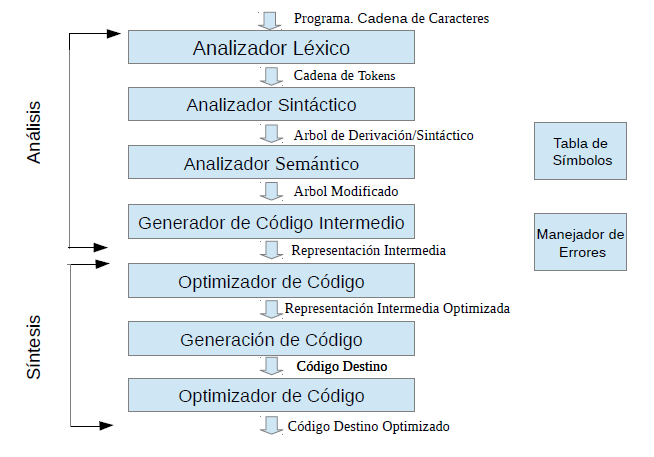
\includegraphics{img/etapas_compilador.png}
}
\caption{Etapas del desarrollo de un compilador, indicando los dos procesos principales.}
\label{fig:etapas}
\end{figure}

El desarrollo tiene dos procesos principales, el \emph{Análisis} y la \emph{Síntesis}. El análisis es el proceso en que se dará énfasis, ya que consta de las etapas más importantes como el análisis léxico, sintáctico y semántico, teniendo principal hincapié en la sintaxis ya que se realizará una \emph{traducción dirigida por la sintaxis} para este trabajo.

En este sentido, para este informe vamos a mostrar el diseño y la implementación de un compilador para un conjunto reducido de construcciones del lenguaje Pascal, explicando el desarrollo de cada etapa y cómo se relaciona con la etapa siguiente.

%\end{adjustwidth*}
\setcounter{page}{1}

\chapter{Gramática del lenguaje}

\section{Introducción}
El diseño y la implementación de un compilador se compone de diferentes etapas, donde cada una requiere una entrada y produce una salida para la etapa siguiente. En este capítulo nos centraremos en la definición preliminar de una gramática para generar las cadenas de entrada que tendrá nuestro lenguaje. En capítulos posteriores utilizaremos estas definiciones para el desarrollo de las etapas siguientes en proceso de compilación.

\section{Descripción del problema}
\label{desc_problema}
Para esta primer etapa, debemos definir cómo va a ser la estructura de las cadenas de entrada del lenguaje. Para esto formalizaremos con una gramática utilizando una notación específica, que veremos en la sección \ref{metalenguaje}. En este sentido, se definirán las siguientes construcciones que serán aceptadas por el compilador:
\begin{itemize}
\item Definición de variables y subprogramas.
\item Tipos de datos simples: se utilizaron datos \textbf{integer} y \textbf{boolean}.
\item Constantes usadas en las expresiones: \textbf{true} y \textbf{false}.
\item Subprogramas: se pueden definir procedimientos y funciones, con pasaje de parámetro por valor.
\item Sentencias:

\begin{itemize}
\item Asignación.
\item Repetitiva: \textbf{while}.
\item Alternativa: \textbf{if then else}.
\item Sentencias compuestas: \textbf{begin end}.
\end{itemize}

\item Procedimientos \textbf{read} y \textbf{write} para un solo valor.
\item Operaciones aritméticas: $+$, $-$, $*$, $/$, con uso de paréntesis. 
\item Operaciones booleanas: operadores \textbf{AND}, \textbf{OR}, \textbf{NOT}, y operadores de comparación: $<=$, $>=$, $>$, $<$, $=$.
\end{itemize}

\section{Metalenguaje}
\label{metalenguaje}
Para expresar el lenguaje se ha utilizado una gramática con la notación \textbf{BNF} sin extender, de manera que se eviten ambigüedades con respecto a las notaciones propuestas por los diferentes autores.

Hemos utilizado la siguiente convención para la definición de la gramática:

\begin{itemize}
\item Los símbolos no terminales van encerrados entre $<$ y $>$.
\item Los símbolos terminales se ven en \textbf{negrita}.
\item Cada regla de producción diferencia su parte izquierda de su parte derecha con el símbolo $\rightarrow$.
\item Las opciones alternativas en cada regla se especifican con el símbolo $|$.
\end{itemize}

\section{Estrategias}
\label{estrategias}
Para definir la gramática hemos tenido en cuenta la propia definición dada para Pascal (que puede encontrarse en la web) y se la ha limitado en varios sentidos expresados en la sección \ref{limitaciones}, como también se ha optimizado para el caso de no terminales inútiles o repetidos, siempre buscando generar una gramática válida.

Por otro lado, como se ha decidido implementarla en \textbf{BNF} sin extender [\ref{metalenguaje}], la gramática quedó expresada utilizando recursividad, lo cual en etapas siguientes permitirá una traducción a código mas directa.

Se ha decidido realizar la gramática considerando optimizar el uso de los no terminales, en vez de tener en cuenta una posible expansión a futuro, es decir, que nuestra definición no será fácilmente adaptable al cambio pero tendrá un mejor rendimiento en el momento de implementarse.

\section{Limitaciones}
\label{limitaciones}
Como se ha mencionado en la sección \ref{desc_problema}, se realizará un compilador para el lenguaje Pascal limitado en varios aspectos. En un principio solo se tendrán en cuenta variables del tipo \textbf{integer} y \textbf{boolean}. Los procedimientos y funciones no podrán recibir parámetros por referencia, solo por valor. Dentro de las sentencias alternativas solo encontraremos \textbf{if then else} y en repetitivas solo la sentencia \textbf{while}. No se tendrá en cuenta parámetros enviados al programa principal. Y finalmente las sentencias de escritura y lectura se verán limitadas a un solo valor, y para la salida se tendrán en cuenta algunas consideraciones [\ref{sec:cons_salida}].

Con respecto a la especificación, debido a que hemos decidido utilizar {\bf BNF} sin extender, este se ve limitado en expresividad, ya que no utilizamos símbolos para  repetitivas, opcionales, agrupaciones, etc. A pesar de esto, creemos que la especificación es clara dado que el lenguaje trabajado no es de gran magnitud.

\subsection{Consideraciones para la salida}
\label{sec:cons_salida}
La instrucción de salida write permite especificar el formato de salida de una variable. El formato depende del tipo de variable que se pase por parámetro. En nuestro caso tenemos solo dos tipos de variables, integer y boolean. Para imprimir estos dos tipos de dato hay que tener en cuenta las siguientes características:

\begin{itemize}
\item{Integer}\\
write(number : fieldwidth);\\
Se reservará un campo de ancho ``fieldwidth'' y ``number'' se justificará a la derecha en este campo, con los lugares restantes a la izquierda llenos de espacios en blanco. Si ``fieldwidth'' no es lo suficientemente grande como para cubrir todos los dígitos de ``number'', se mostrará correctamente en un campo más amplio. ``fieldwidth'' también puede ser una variable o expresión de tipo entero.
\item{Boolean}\\
write(flag : fieldwidth);\\
Esto generará ``verdadero'' o ``falso'' dentro del ancho de campo especificado, si se especifica.
\end{itemize}

El parámetro ``fieldwidth'' es opcional. Para facilitar la implementación no vamos a tener en cuenta esta característica del lenguaje.

\section{Definición de la gramática}
\label{sec:definicion_gramatica}
A continuación se mostrará la definición de la gramática en \textbf{BNF} para el lenguaje enunciado anteriormente. Considerar el símbolo inicial $<$program$>$.

%los terminales van entre "" y se ven en negrita.
%los no terminales van entre <>.
%punto y coma es el alternativo |
%los dos puntos son para la flechita derecha para determinar las partes de una regla.

	\begin{grammar}
		[(colon){$\rightarrow$}]
		[(semicolon)$|$]
		[(comma){}]
		[(period){\vspace{0.3cm} \\}]
		[(quote){\begin{bf}}{\end{bf}}]
		[(nonterminal){$<$}{$>$}]
		
		%<expression> : <number> ; <number>, [\{"asd"\}], <relational\_operator>, <number>.
		%<number> : <digit> ; <digit> , <number>.
		%<digit> : "0";"1";"2";"3";"4";"5";"6";"7";"8";"9".
		%<relational\_operator> : $"="$;"$\lessthan \greaterthan$";"$\lessthan$";"$\greaterthan$"; "$\lessthan=$";"$\greaterthan=$";"in".
		
		<program> : <program-heading> <block> ".".
		<program-heading> : "program" <identifier> ";".
		<block> : <declaration-block> <multiple-statement> ; <multiple-statement>.
		<declaration-block> : <variable-declaration-block> ; <variable-declaration-block> <procedure-and-function-declaration-list> ; <procedure-and-function-declaration-list>.
		<variable-declaration-block> : "var" <variable-declaration-list>.
		<variable-declaration-list> : <variable-declaration> ";" ; <variable-declaration> ";" <variable-declaration-list>.
		<variable-declaration> : <identifier-list> ":" <type>.
		<procedure-and-function-declaration-list> : <procedure-declaration> ";" ; <function-declaration> ";" ; <procedure-declaration> ";" <procedure-and-function-declaration-list> ; <function-declaration> ";" <procedure-and-function-declaration-list>.
		<procedure-declaration> : <procedure-heading> ";" <block>.
		<procedure-heading> : "procedure" <identifier> ; "procedure" <identifier> "("")" ; "procedure" <identifier> "(" <parameter-declaration-list> ")".
		<function-declaration> : <function-heading> ";" <block>.
		<function-heading> : "function" <identifier> ":" <type> ; "function" <identifier> "("")" ":" <type> ; "function" <identifier> "(" <parameter-declaration-list> ")" ":" <type>.
		<parameter-declaration-list> : <parameter-declaration> ; <parameter-declaration> "," <parameter-declaration-list>.
		<parameter-declaration> : <identifier-list> ":" <type>.
        <statement-block> : <statement> ; <multiple-statement>.
		<multiple-statement> : "begin" <statement-list> "end".
		<statement-list> : <statement> ; <statement> ";" <statement-list>.
		<statement> : <simple-statement> ; <structured-statement>.
		<simple-statement> : <assignment-statement> ; <call-procedure-or-function> ; <call-write-read-procedure>.
		<structured-statement> : <conditional-statement> ; <repetitive-statement>.
		<assignment-statement> : <identifier> ":=" <expression>.
		%la segunda alternativa para call-procedure-or-function es para el caso del write.
		<call-procedure-or-function> : <identifier> ; <identifier> "("")" ; <identifier> "(" <expression-list> ")".
        <call-write-read-procedure> : "write" ; "read" ; "write" "("")" ; "read" "("")" ; "write" "(" <expression-list> ")" ; "read" "(" <expression-list> ")". 
		<conditional-statement> : "if" <expression> "then" <statament-block> ; "if" <expression> "then" <statament-block> "else" <statament-block>.
		<repetitive-statement> : "while" <expression> "do" <statement-block>.
		<expression-list> : <expression> ; <expression> "," <expression-list>.
        <expression> :  <expression> "or" <expression$_{1}$> ; <expression$_{1}$>. 
		<expression$_{1}$> :  <expression$_{1}$> "and" <expression$_{2}$>; <expression$_{2}$>.
		<expression$_{2}$> : <expression$_{2}$> <relational-operator> <expression$_{3}$> ; <expression$_{3}$>.
		<expression$_{3}$> : <expression$_{3}$> <addition-operator> <expression$_{4}$> ;  <expression$_{4}$>.
		<expression$_{4}$> : <expression$_{4}$> <multiplication-operator> <expression$_{5}$> ;  <expression$_{5}$>.
		<expression$_{5}$> : <identifier> ; "(" <expression> ")" ; <call-procedure-or-function> ; <unary-operator> <expression$_{5}$> ; <literal>.
		<relational-operator> : "$=$" ; "$<>$" ; "$<$" ; "$<=$" ; "$>$" ; "$>=$".
        <unary-operator> : $-$ ; "not".
		<addition-operator> : "$+$" ; "$-$".
		<multiplication-operator> : "$*$" ; "$/$".
		<type> : "integer" ; "boolean".
		<identifier-list> : <identifier> ; <identifier> "," <identifier-list>.
		<identifier> : <letter> <identifier$_1$> ; \_ <identifier$_1$> .
        <identifier$_1$> : <word> <identifier$_1$> ; <number> <identifier$_1$> ; $\lambda$.
		<literal> : <bool> ; <number>.
		<number> :  <digit> <number$_1$>.
		<number$_1$> : <digit> <number$_1$> ; $\lambda$.
        <word> : <letter> <word$_1$> ; "\_" <word$_1$>.
		<word$_1$> : "\_" <word$_1$> ; <letter> <word$_1$> ; $\lambda$.
		<letter> : "A" ; "B" ; "C" ; "D" ; "E" ; "F" ; "G" ; "H" ; "I" ; "J" ; "K" ; "L" ; "M" ; "N" ; "O" ; "P" ; "Q" ; "R" ; "S" ; "T" ; "U" ; "V" ; "W" ; "X" ; "Y" ; "Z" ; "a" ; "b" ; "c" ; "d" ; "e" ; "f" ; "g" ; "h" ; "i" ; "j" ; "k" ; "l" ; "m" ; "n" ; "o" ; "p" ; "q" ; "r" ; "s" ; "t" ; "u" ; "v" ; "w" ; "x" ; "y" ; "z".
		<digit> : "0" ; "1" ; "2" ; "3" ; "4" ; "5" ; "6" ; "7" ; "8" ; "9".
		<bool> : "true" ; "false".
\end{grammar}

\section{Problemas encontrados}
Como se ha decidido utilizar \textbf{BNF} sin extender, fue necesario reemplazar las notaciones repetitivas, optativas y opcionales, que se tuvieron en cuenta en un principio, por una versión equivalente sin ellas. No se han tenido mayores complicaciones, dada la facilidad y simplicidad que otorga la notación de gramáticas.

\section{Conclusiones}
Se ha logrado realizar una gramática en notación \textbf{BNF} sin extender, que cumpla con los requisitos del problema [\ref{desc_problema}], denotando las limitaciones [\ref{limitaciones}] que tendrá el lenguaje que se compilará y considerando optimizar la gramática de manera que se obtenga un mayor rendimiento en la implementación futura [\ref{estrategias}].

\chapter{Especificación léxica}

\section{Introducción}
En este capítulo utilizaremos la gramática desarrollada en el capítulo anterior y realizaremos el diseño de un analizador léxico. El objetivo es recorrer la cadena de entrada carácter por carácter y detectar los {\bf tokens} especificados, en este caso Pascal reducido (definido por la gramática).
Para ello, se indicarán como están formados los \emph{tokens}, que son elementos que utilizará el analizador sintáctico posteriormente, y se mostrará el diseño de un autómata que permita el reconocimiento de tales tokens en un recorrido [\ref{sec:lexico_reconocedor}].

\section{Descripción del problema}
Para esta etapa requerimos especificar en un principio el alfabeto que tendrá nuestra cadena de entrada, luego debemos definir que combinación de símbolos corresponderán a lexemas de nuestro lenguaje y partir de estos debemos generar patrones que identifiquen para cada token que lexemas les corresponden [\ref{sec:lexico_definicion}].

Dados los tokens y sus patrones representativos, se especifica un autómata finito determinístico que lee cada símbolo de la cadena de entrada y permite determinar si es un token válido del lenguaje. Para ello el autómata se realiza mediante la unión de autómatas más simples para reconocer los patrones de cada token por separado.

\section{Definición del alfabeto, lexemas, tokens y patrones}
\label{sec:lexico_definicion}
El alfabeto estará compuesto por las letras del abecedario (A-Z y a-z) en conjunción con los dígitos de 0-9 y algunos caracteres especiales:

$$ \Sigma = \{ \bm{A}, ..., \bm{Z}, \bm{a}, ..., \bm{z}, \bm{0}, ..., \bm{9}, \bm{\_}, \bm{\}}, \bm{\{}, \bm{)}, \bm{(}, \bm{;}, \bm{\cdot}, \bm{,}, \bm{:}, \bm{=}, \bm{<}, \bm{>}, \bm{+}, \bm{-}, \bm{*}, \bm{/} \}$$

Con estos símbolos podemos definir los lexemas que componen el subconjunto de lenguaje Pascal que se desarrolla y luego definir expresiones regulares para poder identificar a que token corresponden.

En la tabla \ref{tab:tabla_token} podemos visualizar los token que se indentifican en el lenguaje especificado junto con los patrones que definen los lexemas que se corresponden con cada uno de estos token. Tales patrones se especificarán mediante expresiones regulares.

\begin{table}[H]
\centering
\begin{tabular}{|l|l|l|}
\rowcolor{gray!20}
\hline
Token         & Patrón                                               & Ejemplo              \\ \hline
tk\_type\_int      & $integer$                                  & $integer$            \\ \hline
tk\_type\_bool      & $boolean$                                  & $boolean$            \\ \hline
tk\_boolean\_true   & $true$                                       & $true$               \\ \hline
tk\_boolean\_false   & $false$                                       & $false$               \\ \hline
tk\_number   & $[0-9]^+$                                            & $100$                \\ \hline
tk\_id        & $([A-Z] | [a-z] | \_)([A-Z] | [a-z] | \_ | [0-9])^*$ & $un\_identificador\_1$ \\ \hline
tk\_assign    & $:=$                                                 & $:=$                 \\ \hline
tk\_rel\_op\_eq   & $=$                           & $=$                 \\ \hline
tk\_rel\_op\_neq   & $<>$                           & $<>$                 \\ \hline
tk\_rel\_op\_min   & $<$                           & $<$                 \\ \hline
tk\_rel\_op\_may   & $>$                           & $>$                 \\ \hline
tk\_rel\_op\_leq   & $<=$                           & $<=$                 \\ \hline
tk\_rel\_op\_geq   & $>=$                           & $>=$                 \\ \hline
tk\_add\_op\_sum   & $+$                                             & $+$                  \\ \hline
tk\_add\_op\_rest   & $-$                                             & $-$                  \\ \hline
tk\_mult\_op\_por  & $*$                                              & $*$                  \\ \hline
tk\_mult\_op\_div  & $/$                                              & $/$                  \\ \hline
tk\_bool\_op\_and  & $and$                                           & $and$                \\ \hline
tk\_bool\_op\_or  & $or$                                           & $or$                \\ \hline
tk\_not\_op   & $not$                                                & $not$                \\ \hline
tk\_if        & $if$                                                 & $if$                 \\ \hline
tk\_then      & $then$                                               & $then$               \\ \hline
tk\_else      & $else$                                               & $else$               \\ \hline
tk\_while     & $while$                                              & $while$              \\ \hline
tk\_do        & $do$                                                 & $do$                 \\ \hline
tk\_program   & $program$                                            & $program$            \\ \hline
tk\_begin     & $begin$                                              & $begin$              \\ \hline
tk\_end       & $end$                                                & $end$                \\ \hline
tk\_var       & $var$                                                & $var$                \\ \hline
tk\_procedure & $procedure$                                          & $procedure$          \\ \hline
tk\_function  & $function$                                           & $function$           \\ \hline
tk\_read  & $read$                                           & $read$           \\ \hline
tk\_write  & $write$                                           & $write$           \\ \hline
tk\_opar      & (                                                    & (                    \\ \hline
tk\_cpar      & )                                                    & )                    \\ \hline
tk\_tpoints   & :                                                    & :                    \\ \hline
tk\_endstnc   & ;                                                    & ;                    \\ \hline
tk\_point     & .                                                    & .                    \\ \hline
tk\_comma     & ,                                                    & ,                    \\ \hline
\end{tabular}
\caption{Define para cada token el patrón que identifica los lexemas que le corresponden.}
\label{tab:tabla_token}
\end{table}

\section{Estrategias}
Utilizamos diferentes tokens para cada uno de los operadores, como en los operadores de comparación, de multiplicación, y de suma. Así aunque se manejen mas cantidad de tokens que si estuvieren agrupados, es mas sencillo diferenciarlos en las etapas posteriores.

Para componer el reconocedor, tomaremos cualquier cadena de entrada que pueda ser una palabra clave, con el patrón del token id. Si es una palabra clave, se crea su token correspondiente, si no lo es, entonces se confirma que es un id. De esta manera se simplifica el autómata reconocedor de tokens.

\section{Limitaciones}
\label{sec:lexico_limitaciones}
En la especificación de tokens se ha indicado para cada operador un token diferente, como con los operadores relacionales (rel\_op), esto permite diferenciarlos y en futuras etapas facilita la implementación. En cambio se pudo optar por una visión mas genérica que facilite la visualización de los diferentes token conceptualmente, de manera que queden agrupados y se diferencien por un atributo que indique específicamente que lexema representa.

Por otro lado, con respecto al diseño del autómata, se consideró, para simplificar el diseño, que las palabras reservadas no serán reconocidas por estados independientes si no que serán un caso específico del patrón para reconocer identificadores (tk\_id).

\section{Diseño del reconocedor}
\label{sec:lexico_reconocedor}

% \begin{figure}[H]
% \begin{center}
% \begin{tikzpicture}[scale=0.15]
% \tikzstyle{every node}+=[inner sep=0pt]
% \draw [black] (49,-15.4) circle (3);
% \draw (49,-15.4) node {$2$};
% \draw [black] (49,-2.8) circle (3);
% \draw (49,-2.8) node {$1$};
% \draw [black] (64.8,-15.4) circle (3);
% \draw (64.8,-15.4) node {$3\mbox{ }*$};
% \draw (76,-15.4) node {{\bf return($tk\_id$)}};
% \draw [black] (64.8,-15.4) circle (2.4);
% \draw [black] (22.5,-2.8) circle (3);
% \draw (22.5,-2.8) node {$start$};
% \draw [black] (49,-28.4) circle (3);
% \draw (49,-28.4) node {$4$};
% \draw [black] (65.4,-28.4) circle (3);
% \draw (65.4,-28.4) node {$5\mbox{ }*$};
% \draw (78.5,-28.4) node {{\bf return($tk\_integer$)}};
% \draw [black] (65.4,-28.4) circle (2.4);
% \draw [black] (49,-38.3) circle (3);
% \draw (49,-38.3) node {$6$};
% \draw [black] (65.4,-42.6) circle (3);
% \draw (65.4,-42.6) node {$7$};
% \draw (78.5,-42.6) node {{\bf return($tk\_assign$)}};
% \draw [black] (65.4,-42.6) circle (2.4);
% \draw [black] (48.5,-47.4) circle (3);
% \draw (48.5,-47.4) node {$8$};
% \draw (63.4,-46.9) node {{\bf return($tk\_rel\_op\_eq$)}};
% \draw [black] (48.5,-47.4) circle (2.4);
% \draw [black] (48.5,-56.2) circle (3);
% \draw (48.5,-56.2) node {$9$};
% \draw [black] (65.4,-51.7) circle (3);
% \draw (65.4,-51.7) node {$10\mbox{ }*$};
% \draw (80,-51.7) node {{\bf return($tk\_rel\_op\_min$)}};
% \draw [black] (65.4,-51.7) circle (2.4);
% \draw [black] (65.4,-59.1) circle (3);
% \draw (65.4,-59.1) node {$11$};
% \draw (80,-59.1) node {{\bf return($tk\_rel\_op\_leq$)}};
% \draw [black] (65.4,-59.1) circle (2.4);
% \draw [black] (65.4,-66) circle (3);
% \draw (65.4,-66) node {$12$};
% \draw (80,-66) node {{\bf return($tk\_rel\_op\_neq$)}};
% \draw [black] (65.4,-66) circle (2.4);
% \draw [black] (48.5,-72.8) circle (3);
% \draw (48.5,-72.8) node {$13$};
% \draw [black] (65.4,-72.8) circle (3);
% \draw (65.4,-72.8) node {$14$};
% \draw (80,-72.8) node {{\bf return($tk\_rel\_op\_geq$)}};
% \draw [black] (65.4,-72.8) circle (2.4);
% \draw [black] (65.4,-80.7) circle (3);
% \draw (65.4,-80.7) node {$15\mbox{ }*$};
% \draw (80,-80.7) node {{\bf return($tk\_rel\_op\_may$)}};
% \draw [black] (65.4,-80.7) circle (2.4);
% \draw [black] (49,-86.4) circle (3);
% \draw (49,-86.4) node {$16$};
% \draw (63,-86.4) node {{\bf return($tk\_add\_op$)}};
% \draw [black] (49,-86.4) circle (2.4);
% \draw [black] (49,-95.6) circle (3);
% \draw (49,-95.6) node {$18$};
% \draw (63,-95.6) node {{\bf return($tk\_mult\_op$)}};
% \draw [black] (49,-95.6) circle (2.4);
% \draw [black] (65.4,-35.7) circle (3);
% \draw (65.4,-35.7) node {$19\mbox{ }*$};
% \draw (78.5,-35.7) node {{\bf return($tk\_tpoins$)}};
% \draw [black] (65.4,-35.7) circle (2.4);
% \draw [black] (51.253,-0.837) arc (158.78564:-129.21436:2.25);
% \draw (56.29,-0.58) node [right] {$otro$};
% \fill [black] (51.93,-3.39) -- (52.49,-4.15) -- (52.86,-3.22);
% \draw [black] (47.677,-12.72) arc (234:-54:2.25);
% \draw (49,-8.15) node [above] {$letter\mbox{ }or\mbox{ }digit\mbox{ }or\mbox{ }\_$};
% \fill [black] (50.32,-12.72) -- (51.2,-12.37) -- (50.39,-11.78);
% \draw [black] (52,-15.4) -- (61.8,-15.4);
% \fill [black] (61.8,-15.4) -- (61,-14.9) -- (61,-15.9);
% \draw (56.9,-14.9) node [above] {$otro$};
% \draw [black] (46,-2.8) -- (25.5,-2.8);
% \fill [black] (25.5,-2.8) -- (26.3,-3.3) -- (26.3,-2.3);
% \draw (35.75,-3.3) node [below] {$\}$};
% \draw [black] (25.231,-1.562) arc (111.4063:68.5937:28.821);
% \fill [black] (46.27,-1.56) -- (45.71,-0.8) -- (45.34,-1.74);
% \draw (35.75,0.93) node [above] {$\{$};
% \draw [black] (25.21,-4.09) -- (46.29,-14.11);
% \fill [black] (46.29,-14.11) -- (45.78,-13.32) -- (45.35,-14.22);
% \draw (31.15,-9.63) node [below] {$letter\mbox{ }or\mbox{ }\_$};
% \draw [black] (46.059,-27.813) arc (-103.99149:-164.0292:31.782);
% \fill [black] (46.06,-27.81) -- (45.4,-27.13) -- (45.16,-28.1);
% \draw (29.31,-20.31) node [below] {$digit$};
% \draw [black] (47.677,-25.72) arc (234:-54:2.25);
% \draw (49,-21.15) node [above] {$digit$};
% \fill [black] (50.32,-25.72) -- (51.2,-25.37) -- (50.39,-24.78);
% \draw [black] (52,-28.4) -- (62.4,-28.4);
% \fill [black] (62.4,-28.4) -- (61.6,-27.9) -- (61.6,-28.9);
% \draw (57.2,-28.9) node [below] {$otro$};
% \draw [black] (46.002,-38.324) arc (-92.79513:-193.72375:26.42);
% \fill [black] (46,-38.32) -- (45.23,-37.79) -- (45.18,-38.78);
% \draw (25.54,-29.13) node [left] {$:$};
% \draw [black] (51.9,-39.06) -- (62.5,-41.84);
% \fill [black] (62.5,-41.84) -- (61.85,-41.15) -- (61.6,-42.12);
% \draw (58,-39.88) node [above] {$=$};
% \draw [black] (45.501,-48.422) arc (-92.52263:-208.09592:29.287);
% \fill [black] (45.5,-48.42) -- (44.72,-47.89) -- (44.68,-48.89);
% \draw (20.69,-34.89) node [left] {$=$};
% \draw [black] (45.517,-56.504) arc (-86.95094:-221.12695:31.119);
% \fill [black] (45.52,-56.5) -- (44.69,-56.05) -- (44.74,-57.05);
% \draw (15.18,-40.13) node [left] {$<$};
% \draw [black] (51.4,-55.43) -- (62.5,-52.47);
% \fill [black] (62.5,-52.47) -- (61.6,-52.19) -- (61.86,-53.16);
% \draw (55.34,-53.32) node [above] {$otro$};
% \draw [black] (51.46,-56.71) -- (62.44,-58.59);
% \fill [black] (62.44,-58.59) -- (61.74,-57.96) -- (61.57,-58.95);
% \draw (56.46,-58.25) node [below] {$=$};
% \draw [black] (51.1,-57.7) -- (62.8,-64.5);
% \fill [black] (62.8,-64.5) -- (62.36,-63.66) -- (61.86,-64.53);
% \draw (55.89,-61.6) node [below] {$>$};
% \draw [black] (45.516,-72.502) arc (-97.80406:-221.44306:40.861);
% \fill [black] (45.52,-72.5) -- (44.79,-71.9) -- (44.66,-72.89);
% \draw (12,-47.06) node [left] {$>$};
% \draw [black] (51.5,-72.8) -- (62.4,-72.8);
% \fill [black] (62.4,-72.8) -- (61.6,-72.3) -- (61.6,-73.3);
% \draw (56.95,-73.3) node [below] {$=$};
% \draw [black] (51.22,-74.07) -- (62.68,-79.43);
% \fill [black] (62.68,-79.43) -- (62.17,-78.64) -- (61.75,-79.54);
% \draw (54.87,-77.27) node [below] {$otro$};
% \draw [black] (46.068,-85.769) arc (-103.8764:-220.94786:49.664);
% \fill [black] (46.07,-85.77) -- (45.41,-85.09) -- (45.17,-86.06);
% \draw (9.87,-53.22) node [left] {$+\mbox{ }or\mbox{ }-$};
% \draw [black] (46.027,-95.204) arc (-99.23615:-228.88937:51.996);
% \fill [black] (46.03,-95.2) -- (45.32,-94.58) -- (45.16,-95.57);
% \draw (3.61,-58.72) node [left] {$*\mbox{ }or\mbox{ }/$};
% \draw [black] (19.572,-3.399) arc (309.29645:21.29645:2.25);
% \draw (15.21,-0.59) node [left] {$ws$};
% \fill [black] (20.24,-0.84) -- (20.12,0.1) -- (19.35,-0.54);
% \draw [black] (51.96,-37.83) -- (62.44,-36.17);
% \fill [black] (62.44,-36.17) -- (61.57,-35.8) -- (61.73,-36.79);
% \draw (56.34,-36.3) node [above] {$otro$};
% \end{tikzpicture}
% \end{center}
% \caption{Autómata reconocedor de tokens.}
% \label{fig:automata_token2}
% \end{figure}

\begin{figure}[H]
\centering
\begin{tikzpicture}[scale=0.65, node distance = 2.5cm, state/.style={circle, draw, minimum size=1cm}]
\tikzset{every state/.append style={thick, fill=gray!10}}
\node[state] (0) at (0,0) {$start$};
\node[state] (1) at (0,-6) {$1$};
\node[state] (2) at (3,6) {$2$};
\node[state, accepting] (3) at (6,6) {$3$ $*$};
\node[state] (4) at (3,2) {$4$};
\node[state, accepting] (5) at (6,4) {$5$ $*$};
\node[state] (6) at (3,0) {$6$};
\node[state, accepting] (7) at (6,2) {$7$ $*$};
\node[state, accepting] (8) at (6,0) {$8$};
\node[state] (9) at (3,-4) {$9$};
\node[state, accepting] (10) at (6,-2) {$10$ $*$};
\node[state, accepting] (11) at (6,-4) {$11$};
\node[state, accepting] (12) at (6,-6) {$12$};
\node[state] (13) at (-3,5) {$13$};
\node[state, accepting] (14) at (-6,6) {$14$ $*$};
\node[state, accepting] (15) at (-6,4) {$15$};
\node[state, accepting] (16) at (-6,2) {$16$};
\node[state, accepting] (17) at (-6,0) {$17$};
\node[state, accepting] (18) at (-6,-2) {$18$};
\node[state, accepting] (19) at (-6,-4) {$19$};
\node[state, accepting] (20) at (-6,-6) {$20$};

\node[right] at (7,6) {{\bf return($tk\_id$)}};
\node[right] at (7,4) {{\bf return($tk\_number$)}};
\node[right] at (7,2) {{\bf return($tk\_tpoints$)}};
\node[right] at (7,0) {{\bf return($tk\_assign$)}};
\node[right] at (7,-2) {{\bf return($tk\_rel\_op\_min$)}};
\node[right] at (7,-4) {{\bf return($tk\_rel\_op\_leq$)}};
\node[right] at (7,-6) {{\bf return($tk\_rel\_op\_neq$)}};

\node[left] at (-7,6) {{\bf return($tk\_rel\_op\_may$)}};
\node[left] at (-7,4) {{\bf return($tk\_rel\_op\_geq$)}};
\node[left] at (-7,2) {{\bf return($tk\_rel\_op\_eq$)}};
\node[left] at (-7,0) {{\bf return($tk\_add\_op\_sum$)}};
\node[left] at (-7,-2) {{\bf return($tk\_add\_op\_rest$)}};
\node[left] at (-7,-4) {{\bf return($tk\_mult\_op\_por$)}};
\node[left] at (-7,-6) {{\bf return($tk\_mult\_op\_div$)}};

\path[->,>=stealth]
(0) edge[loop above] node{$ws$} (0)	
	edge[bend left, left] node{$\{$} (1)
    edge[above] node{$letter$ or $\_$} (2)
    edge[above] node{$digit$} (4)
    edge[above] node{$:$} (6)
    edge[above] node{$<$} (9)
    edge[left] node{$>$} (13)
    edge[above] node{$=$} (16)
    edge[above] node{$+$} (17)
    edge[above] node{$-$} (18)
    edge[above] node{$*$} (19)
    edge[above] node{$/$} (20)
(1) edge[loop below] node{$otro$} (1)
	edge[bend left, right] node{$\}$} (0)
(2) edge[loop above] node{$letter$ or $digit$ or $\_$} (2)
	edge[above] node{$otro$} (3)
(4) edge[loop above] node{$digit$} (4)
	edge[above] node{$otro$} (5)
(6) edge[above] node{$otro$} (7)
	edge[above] node{$=$} (8)
(9) edge[above] node{$otro$} (10)
	edge[above] node{$=$} (11)
	edge[above] node{$>$} (12)
(13) edge[above] node{$otro$} (14)
	 edge[above] node{$=$} (15)
;
\end{tikzpicture}
\caption{Autómata reconocedor de tokens.}
\label{fig:automata_token}
\end{figure}

Podemos contemplar que en ciertos estados se consume un elemento \emph{otro}, el cuál dependerá de tal estado, y simboliza un elemento que no corresponde con los símbolos cuyos lexemas están incluidos en el patrón del token que está reconociendo. Por ejemplo, en el arco del estado 2-3, \emph{otro} corresponde a símbolos que no son \emph{letter}, \emph{digit} o \emph{\_}. En el caso del arco 4-5 corresponde un símbolo que no es \emph{digit}. En 9-10 para cualquier símbolo que no es \emph{=} o \emph{$>$} y en 13-15 para cualquiera que no sea \emph{=}. Finalmente en el arco del estado 1, se utiliza de manera que reconozca cualquier símbolo, ya que este es el encargado de reconocer las secciones comentadas del código, lo que permite ignorar cualquier símbolo encerrado entre llaves.

Por otro lado, encontramos el arco etiquetado con \emph{ws} que permite ignorar los espacios, los saltos de línea y las tabulaciones.

A modo de simplificación del gráfico, tanto por cuestiones de tamaño como de estética, no se indicó el reconocimiento de los siguientes tokens: tk\_opar, tk\_cpar, tk\_tpoints, tk\_endstnc, tk\_point, tk\_comma. Estos patrones son triviales, y serían análogos, por ejemplo, al reconocimiento de tk\_mult\_op.
%\section{Problemas encontrados}

\section{Implementación del aplicativo}
\label{sec:implementacion_lexico}
En esta sección proponemos una implementación de un analizador léxico que se corresponde con la especificación léxica de la sección anterior.

Se dispondrá el enlace del código fuente alojado en GitHub\footnote{\url{https://github.com/Martinnqn/CompiladorPascal}}. Durante el desarrollo de este trabajo se ampliará el aplicativo con las demás etapas de análisis sintáctico y semántico. De esta manera, esperamos concluir todas las etapas del compilador para el lenguaje elegido.  

\subsection{Descripción del problema}
La idea es desarrollar y documentar un programa capaz de reconocer lexemas de un código fuente basado en la gramática de la sección \ref{sec:definicion_gramatica}, y devolver sus tokens asociados en la tabla \ref{tab:tabla_token}. Para esto, usaremos el autómata de la figura \ref{fig:automata_token}.

\subsection{Herramientas utilizadas} %ver titulo..
Para desarrollar el programa escogimos el lenguaje Java. La versión de Java sobre la que trabajamos es la 8\footnote{Actualización 171, al día 14/05/2018}(ocho), sobre el sistema operativo Windows 10. 

El código de fuente alojado en GitHub tiene la estructura de un proyecto de NetBeans, por lo que puede usarse ese IDE para levantar el proyecto.

\subsection{Diseño}
Para llevar a cabo lo propuesto en este capítulo, y luego poder continuar con el mismo proyecto ampliando el código con las siguientes etapas de análisis, propusimos estructurar el proyecto en \emph{packages}. La estructura del proyecto se puede ver en la figura \ref{fig:arbol_dir}, por lo que ahora nos centraremos en trabajar sobre el paquete \emph{lexico}, el cual contiene todas las clases que se usarán en el análisis léxico.

\begin{figure}[H]
%no borrar el % de dirtree porque es necesario.
\dirtree{%
.1 src.
.2 compiladorpascal.
.3 CompiladorPascal.java.
.3 lexico.
.3 sintactico.
.3 semantico.
}
\caption{Árbol de directorios del proyecto de Java.}
\label{fig:arbol_dir}
\end{figure}
La clase {\bf CompiladorPascal} será la clase principal del proyecto, donde se crearan los objetos necesarios en cada etapa del análisis. 

Las clases que se usarán en el análisis léxico son: {\bf AnalizadorLexico, Token, Tokens}. El árbol de directorios actualizado queda como el de la figura \ref{fig:arbol_dir_2}:
\begin{figure}[H]
%no borrar el % de dirtree porque es necesario.
\dirtree{%
.1 src.
.2 compiladorpascal.
.3 CompiladorPascal.java.
.3 lexico.
.4 AnalizadorLexico.java.
.4 Token.java.
.4 Tokens.java.
.3 sintactico.
.3 semantico.
}
\caption{Árbol de directorios del proyecto de Java con los archivos del analizador léxico.}
\label{fig:arbol_dir_2}
\end{figure}

{\bf Descripción de las clases}: 
\begin{itemize}
\item {\bf AnalizadorLexico}: contiene el código necesario para reconocer cada token y reportar los errores léxicos en caso de haberlos. El código tiene una relación directa con el autómata de la figura \ref{fig:automata_token}.
%\item {\bf ErrorLéxico}: contiene atributos necesarios para mostrar mensajes detallados acerca de los errores léxicos que ocurran durante la compilación. Para cada error se sugiere un mensaje apropiado que permita al programador encontrar el error en el código y poder solucionarlo. 
\item {\bf Token}: contiene los atributos que representan un token, tal como su nombre y valor.
\item {\bf Tokens}: contiene métodos estáticos que almacenan en HashMaps los nombres y valores de los tokens como palabras reservadas y símbolos. Se utilizará en el AnalizadorLexico para obtener los nombres y patrones de los token del lenguaje.
\end{itemize}

%\subsubsection{Estrategias}

%\subsubsection{Limitaciones}

%\subsubsection{Problemas encontrados}

\subsection{Instructivos de instalación y uso}
Al ser un programa hecho en Java, cuenta con la capacidad de ser portable, por lo que no requiere instalación.

El proceso de compilación puede realizarse mediante un IDE (NetBeans en nuestro caso), o mediante la consola o terminal, con el comando \emph{javac *.java} sobre los archivos del paquete.   

\subsection{Ejemplos}
En la figura \ref{fig:lexico_ej_correcto} vemos un programa en nuestro Pascal que es léxicamente correcto, por lo que la salida en la figura \ref{fig:lexico_ej_correcto_salida} nos muestra una cadena con los tokens obtenidos tras el análisis y no menciona ningún error encontrado. Por otro lado en las figura \ref{fig:lexico_ej_error_1} encontramos un código con un caracter desconocido ``$\%$'' y en la figura \ref{fig:lexico_ej_error_1_salida} la correspondiente salida con el error, indicando la línea y posición donde ocurrió y más abajo los tokens que reconoció hasta alcanzar el error. También podemos ver en la figura \ref{fig:lexico_ej_error_2} un código donde no se cierra el comentario por lo que en la figura \ref{fig:lexico_ej_error_2_salida} vemos que la salida es un error específico para este caso.

\begin{figure}[H]
\begin{minted}[autogobble,linenos,xleftmargin=0.35\textwidth,xrightmargin=0.35\textwidth]{pascal}
Program Example1;
Var       
    Num1, Num2, Sum : Integer;
    Result: Boolean;
Begin {no semicolon}
    Sum := Num1 + Num2;
    if (Num1 > Num2) then
        Result := true
End.
\end{minted}
\caption{Programa en Pascal reducido léxicamente correcto.}
\label{fig:lexico_ej_correcto}
\end{figure}

\begin{figure}[H]
\centering
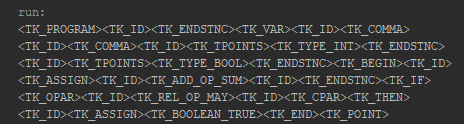
\includegraphics[scale=1]{img/lexico/salida_lexico_ej_correcto.png}
\caption{Salida de la ejecución del analizador léxico con el código de la figura \ref{fig:lexico_ej_correcto}.}
\label{fig:lexico_ej_correcto_salida}
\end{figure}

\begin{figure}[H]
\begin{minted}[autogobble,linenos,xleftmargin=0.35\textwidth,xrightmargin=0.35\textwidth]{pascal}
Program Example2;
Var       
    %Num1, Num2, Sum : Integer;
    Result: Boolean;
Begin [ {no semicolon}
    Sum := Num1 ++ Num2;
    if (Num1 > Num2) then
        Result := true
]
End.
\end{minted}
\caption{Programa en Pascal con error léxico por caracter desconocido.}
\label{fig:lexico_ej_error_1}
\end{figure}

\begin{figure}[H]
\centering
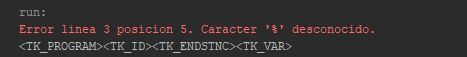
\includegraphics[scale=1]{img/lexico/salida_lexico_ej_error_1.png}
\caption{Salida de la ejecución del analizador léxico con el código de la figura \ref{fig:lexico_ej_error_1}.}
\label{fig:lexico_ej_error_1_salida}
\end{figure}

\begin{figure}[H]
\begin{minted}[autogobble,linenos,xleftmargin=0.35\textwidth,xrightmargin=0.35\textwidth]{pascal}
Program Example3;
Var       
    Num1, Num2, Sum : Integer;
    Result: Boolean;
Begin {no semicolon}
    {Sum := Num1 + Num2;
    if (Num1 > Num2) then
        Result := true
End.
\end{minted}
\caption{Programa en Pascal con error léxico por no encontrar final de comentario.}
\label{fig:lexico_ej_error_2}
\end{figure}

\begin{figure}[H]
\centering
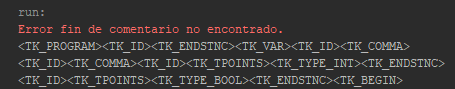
\includegraphics[scale=1]{img/lexico/salida_lexico_ej_error_2.png}
\caption{Salida de la ejecución del analizador léxico con el código de la figura \ref{fig:lexico_ej_error_2}.}
\label{fig:lexico_ej_error_2_salida}
\end{figure}

\section{Conclusiones}
%Realizamos una especificación del autómata de una manera simplificada de manera que sea mas visible su funcionamiento [\ref{sec:lexico_reconocedor}] y a futuro se dará mas detalle a la hora de implementar. De la misma manera para la definición de los token en la tabla \ref{tab:tabla_token} se consideró cada token de una manera mas conceptual y por ello no se especificó uno separado para cada lexema, como se menciona en \ref{sec:lexico_limitaciones}. En este sentido la especificación dada en este capítulo tiene una visión mas general del funcionamiento de un analizador léxico y no tan allegada a la implementación.
En este capítulo pudimos concluir la especificación e implementación del análisis léxico.

Realizamos una definición de los token en la tabla \ref{tab:tabla_token}, considerando cada token conceptualmente como se menciona en \ref{sec:lexico_limitaciones} y así evitamos una definición exhaustiva y simplificamos la tabla.

En base a la tabla de tokens, diseñamos el autómata reconocedor de tokens [\ref{sec:lexico_reconocedor}] describiendo su funcionamiento.

Luego, en la sección \ref{sec:implementacion_lexico}, tuvimos en cuenta las especificaciones y desarrollamos un programa en Java que permite reconocer los tokens de nuestro lenguaje.

En los siguientes capítulos continuaremos desarrollando las especificaciones e implementaciones de las siguientes etapas de un compilador.

\chapter{Especificación sintáctica}

\section{Introducción}
El objetivo de este capítulo es realizar la especificación sintáctica del lenguaje y mostrar un pseudocódigo de su implementación.

Para llevar acabo la especificación sintáctica, trabajaremos sobre algunos aspectos de la gramática de la sección \ref{sec:definicion_gramatica}, realizando modificaciones que permitan implementar un analizador sintáctico descendente predictivo recursivo sin backtracing.

Luego se hará la implementación en lenguaje Java, haciendo uso del Analizador Léxico del capítulo anterior.

\section{Descripción del problema}
Se requiere realizar una modificación sobre la gramática del lenguaje dada en los capítulos anteriores de manera que se obtenga una gramática equivalente que pueda ser utilizada para desarrollar un analizador sintáctico descendente predictivo recursivo. Para ello, la gramática resultante debe estar factorizada a izquierda, no tener recursividad a izquierda y no debe ser ambigua.

Una vez obtenida la gramática y tratados los posibles conflictos se debe proceder en el diseño de una analizador sintáctico que permite evaluar si una cadena de tokens obtenidos mediante el analizador léxico cumple correctamente con la sintaxis dada en la gramática.

\section{Conflictos de la gramática y el lenguaje}
El análisis sintáctico predictivo recursivo es un método top-down de análisis en el que se ejecutan un conjunto de procedimientos recursivos para procesar la entrada.

Para ello se asocia un procedimiento para cada no terminal de la gramática del lenguaje. Al ser un proceso determinístico, se requiere que la gramática a implementar cumpla con ciertas características para evitar conflictos en el desarrollo del analizador:
\begin{itemize}
\item {\bf Gramática factorizada a izquierda:} exige que solo exista un camino para elegir en un no terminal. Ejemplo de una regla de producción no factorizada a izquierda: $<$A$>$ $\rightarrow$ $<$S$>$ $\alpha$ $|$ $<$S$>$ $\beta$.
\item {\bf Gramática sin recursión a izquierda:} hay dos tipos de recursión a izquierda que deben evitarse: 
\begin{itemize}
\item Cuando se da de manera inmediata en la misma regla de producción: 
\begin{center}
$<$A$>$ $\rightarrow$ $<$A$>$ $\alpha$ $|$ $\beta$
\end{center}
\item Cuando se da a partir de varias reglas de producción:
\begin{center}
$<$S$>$ $\rightarrow$ $<$A$>$ $\beta$\\
$<$A$>$ $\rightarrow$ $<$S$>$ $\alpha$ $|$ $\alpha$
\end{center}
\end{itemize}
\item {\bf Gramática no ambigua:} que exista un único árbol de derivación para una entrada.
\end{itemize}

Las gramáticas que cumplen con estas características son clasificadas en las clases de gramática LL(1). A continuación trataremos de modificar nuestra gramática para que alcance la clase de gramáticas LL(1) o resuelvan estos conflictos mediante un tratamiento especial.

\subsection{Factorización a izquierda}
Para factorizar a izquierda se utilizó el siguiente algoritmo:

\begin{center}
\fbox{\begin{minipage}{14cm}
Sea la regla sin factorización a izquierda:
\begin{center}
$<$A$>$ $\rightarrow$ $\alpha$ $|$ $\alpha$ $<$B$>$
\end{center}
Se procede a reemplazarla por la siguiente construcción, factorizada izquierda, equivalente:
\begin{center}
$<$A$>$ $\rightarrow$ $\alpha$ $<$A$_1$$>$ \\
$<$A$_1$$>$ $\rightarrow$ $<$B$>$ $|$ $\lambda$
\end{center}
Donde $<$A$_1$$>$ es un nuevo no terminal que se genera.
\end{minipage}}
\end{center}

Las reglas a las que se les aplicó la factorización a izquierda se presentan en la lista \ref{list:fac_izq} (para simplificar la lista solo pondremos los no terminales del lado izquierdo de la regla):
\begin{mylist}[H]
\caption{Reglas a las que se le aplica factorización a izquierda.}
\begin{multicols}{3}
\begin{itemize}
\item $<$declaration-block$>$
\item $<$variable-declaration-list$>$
\item $<$procedure-and-function-declaration-list$>$
\item $<$procedure-heading$>$ 
\item $<$function-heading$>$
\item $<$parameter-declaration-list$>$
\item $<$statement-list$>$
\item $<$call-write-read-procedure$>$
\item $<$conditional-statement$>$
\item $<$expression-list$>$
\item $<$identifier-list$>$
\end{itemize}
\end{multicols}
\label{list:fac_izq}
\end{mylist}

A modo de ejemplo mostraremos cómo aplicar este método a la regla  $<$statement-list$>$.

\begin{center}
\fbox{\begin{minipage}{14cm}
Sea la regla no factorizada a izquierda: 
\begin{center}
$<$statement-list$>$ $\rightarrow$ $<$statement$>$ $|$ $<$statement$>$ {\bf ;} $<$statement-list$>$
\end{center}
El resultado tras factorizarla a izquierda es:
\begin{center}
$<$statement-list$>$ $\rightarrow$ $<$statement$>$ $<$statement-list$_1$$>$ \\
$<$statement-list$_1>$ $\rightarrow$ {\bf ;} $<$statement-list$>$ $|$ $\lambda$.
\end{center}
Donde $<$statement-list$_1$$>$ es el nuevo no terminal que se genera con la aplicación del método.
\end{minipage}}
\end{center}

Esto fue aplicado a todas las reglas descritas en la lista \ref{list:fac_izq}.

\subsection{Quitando recursión a izquierda}
Para eliminar la recursión a izquierda se utilizó el siguiente método:

\begin{center}
\fbox{\begin{minipage}{14cm}
Sea la regla con recursión a izquierda inmediata:
\begin{center}
$<$A$>$ $\rightarrow$ $<$A$>$ $\alpha$ $|$ $\beta$
\end{center}
Se procede a reemplazarla por la siguiente construcción, sin recursión a izquierda, equivalente:
\begin{center}
$<$A$>$ $\rightarrow$ $\beta$ $<$A$_1$$>$ \\
$<$A$_1$$>$ $\rightarrow$ $\alpha$ $<$A$_1$$>$ $|$ $\lambda$ 
\end{center}
Donde $<$A$_1$$>$ es un nuevo no terminal.
\end{minipage}}
\end{center}

Las reglas que fueron modificadas para eliminar la recursión a izquierda se presentan en la lista \ref{list:rec_izq} (para simplificar la lista solo pondremos los no terminales del lado izquierdo de la regla):

\begin{mylist}[H]
\caption{Reglas a las que se le elimina la recursión a izquierda.}
\begin{multicols}{3}
\begin{itemize}
\item $<$expression$>$.
\item $<$expression$_1$$>$.
\item $<$expression$_2$$>$.
\item $<$expression$_3$$>$.
\item $<$expression$_4$$>$.
\item $<$expression$_5$$>$.
\end{itemize}
\end{multicols}
\label{list:rec_izq}
\end{mylist}

A modo de ejemplo mostraremos cómo aplicar este método a la regla principal desde la cual comienzan a generarse las expresiones. Como se generan muchos no terminales adicionales, primero cambiamos los nombres para que sean más significativos:
\begin{itemize}
\item $<$expression$>$ fue cambiado por $<$expression-or$>$
\item $<$expression$_1$$>$ fue cambiado por $<$expression-and$>$
\item $<$expression$_2$$>$ fue cambiado por $<$expression-rel$>$
\item $<$expression$_3$$>$ fue cambiado por $<$expression-add$>$
\item $<$expression$_4$$>$ fue cambiado por $<$expression-mult$>$
\item $<$expression$_5$$>$ fue cambiado por $<$factor$>$
\end{itemize}

Ahora mostraremos cómo es el resultado de aplicar el método:

\begin{center}
\fbox{\begin{minipage}{14cm}
Sea la regla con recursividad a izquierda:
\begin{center}
$<$expression-or$>$ $\rightarrow$  $<$expression-or$>$ ``or'' $<$expression-and$>$ $|$ $<$expression-and$>$
\end{center}
El resultado tras quitar la recursión a izquierda es:
\begin{center}
$<$expression-or$>$ $\rightarrow$ $<$expression-and$>$ $<$expression-or$_1$$>$ \\
$<$expression-or$_1$$>$ $\rightarrow$ ``or'' $<$expression-and$>$ $<$expression-or$_1$$>$ $|$ $\lambda$.
\end{center}
Donde $<$expression-or$_1$$>$ es el nuevo no terminal que se genera con la aplicación del método.
\end{minipage}}
\end{center}

Esto fue aplicado a todas las reglas descritas en la lista \ref{list:rec_izq}

\subsection{Ambigüedad del lenguaje}
\label{sec:ambiguedad_lenguaje}
La ambigüedad surge cuando existe más de una forma de derivar una cadena. En este lenguaje, cuando se generan construcciones que contienen \texttt{if-then-else} anidados, se pueden generar dos árboles diferentes de derivación. En las figuras \ref{fig:arbol_sintatico_if_ambiguo_1} y \ref{fig:arbol_sintatico_if_ambiguo_2} se ven los árboles posibles para la derivación del siguiente fragmento de programa en nuestro lenguaje:
\begin{figure}[H]
\begin{minted}[autogobble,linenos,xleftmargin=0.35\textwidth,xrightmargin=0.35\textwidth]{pascal}
	if (cond_1) then
		if (cond_2) then
			code_then
		else
			code_else
\end{minted}
\caption{Fragmento de código con \texttt{if} anidados.}
\label{fig:if_ambiguo}
\end{figure}

\begin{figure}[H]
\centering
\begin{tikzpicture}[sibling distance=8em,every node/.style = {shape=rectangle, rounded corners,draw, align=center, scale=0.85}]]
\node {conditional-statement}
	child { node {if} }
	child { node {expression-or}
		child { node {...} 
        	child { node {cond\_1} }
        }
	}
	child { node {then} }
    child { node {statement-block} 
    	child { node {statement} 
        	child { node {structured-statement} 
            	child { node {conditional-statement} 
                	child { node {if} }
                    child { node {expression-or}
                    	child { node {...}
                    		child { node {cond\_2} }
                        }
					}
                    child { node {then} }
                    child { node {statement-block}
                    	child { node {...} 
                    		child { node {code\_then} }
                        }
					}
                    child { node {else-statement} 
                    	child { node {$\lambda$} } 
					}
				}
			}
		}
	}
    child { node {else-statement}
    	child { node {else} }
		child { node {statement-block}
        	child { node {...}
        		child { node {code\_else} }
            }
        } 
	};
\end{tikzpicture}
\caption{Árbol de derivación $A$ para la construcción \texttt{if-then-else}.}
\label{fig:arbol_sintatico_if_ambiguo_1}
\end{figure}

\begin{figure}[H]
\centering
\begin{tikzpicture}[sibling distance=8.25em,every node/.style = {shape=rectangle, rounded corners,draw, align=center, scale=0.85}]]
\node {conditional-statement}
	child { node {if} }
	child { node {expression-or}
    	child { node {...}
			child { node {cond\_1} } 
        }
	}
	child { node {then} }
    child { node {statement-block} 
    	child { node {statement} 
        	child { node {structured-statement} 
            	child { node {conditional-statement} 
                	child { node {if} }
                    child { node {expression-or}
                    	child { node {...}
                    		child { node {cond\_2} }
                        }
					}
                    child { node {then} }
                    child { node {statement-block}
                    	child { node {...}
                    		child { node {code\_then} }
                        }
					}
                    child { node {else-statement}
   					 	child { node {else} }
						child { node {statement-block}
                        	child { node {...}
        						child { node {code\_else} }
                            }
        				} 
					}
				}
			}
		}
	}
    child { node {else-statement}
		child { node {$\lambda$} } 
	};
\end{tikzpicture}
\caption{Árbol de derivación $B$ para la construcción \texttt{if-then-else}.}
\label{fig:arbol_sintatico_if_ambiguo_2}
\end{figure}

El problema surge al momento de decidir si el código correspondiente al \texttt{else} se corresponde con el \texttt{if} interno o el externo.
Este inconveniente no permite que la gramática alcance la clase de gramáticas LL(1). Sin embargo, se puede forzar la implementación del analizador sintáctico para que tome por un camino específico cuando se encuentra esta construcción. La forma más natural es la de la figura \ref{fig:arbol_sintatico_if_ambiguo_2}, donde se asocia el \texttt{else} al \texttt{if} más interno en la estructura de \texttt{if} anidados. Esta es la forma que adoptaremos en la implementación de nuestro analizador.

\section{Gramática modificada}
\label{sec:gramatica_mod}
En esta sección se muestra la gramática con las modificaciones que fueron posibles realizar. 

Se eliminó la recursión a izquierda inmediata y también se factorizó a izquierda. 

Además se eliminó un problema que surgía en el no terminal $<$expression$_{5}$$>$, ya que desde este se podía derivar en $<$identifier$>$ y en $<$call-procedure-or-function$>$, y este último también derivaba en $<$identifier$>$, lo que ocasionaba problemas de factorización a izquierda.

El único inconveniente es que no es posible eliminar la ambigüedad, ya que esta es inherente al lenguaje que está siendo especificado. En la sección \ref{sec:ambiguedad_lenguaje} se mostró dónde surge la ambigüedad.
 
\begin{grammar}
		[(colon){$\rightarrow$}]
		[(semicolon)$|$]
		[(comma){}]
		[(period){\vspace{0.3cm} \\}]
		[(quote){\begin{bf}}{\end{bf}}]
		[(nonterminal){$<$}{$>$}]
		
		%<expression> : <number> ; <number>, [\{"asd"\}], <relational\_operator>, <number>.
		%<number> : <digit> ; <digit> , <number>.
		%<digit> : "0";"1";"2";"3";"4";"5";"6";"7";"8";"9".
		%<relational\_operator> : $"="$;"$\lessthan \greaterthan$";"$\lessthan$";"$\greaterthan$"; "$\lessthan=$";"$\greaterthan=$";"in".
		
		<program> : <program-heading> <block> ".".
		<program-heading> : "program" <identifier> ";".
		<block> : <declaration-block> <multiple-statement> ; <multiple-statement>.
		<declaration-block> : <variable-declaration-block> <declaration-block$_1$> ; <declaration-block$_1$>.
        <declaration-block$_1$> : <procedure-and-function-declaration-list> ; $\lambda$.
		<variable-declaration-block> : "var" <variable-declaration-list>.
		<variable-declaration-list> : <variable-declaration> ";" <variable-declaration-list$_1$>.
        <variable-declaration-list$_1$> : <variable-declaration-list> ; $\lambda$.
		<variable-declaration> : <identifier-list> ":" <type>.
		<procedure-and-function-declaration-list> : <procedure-declaration> ";" <procedure-and-function-declaration-list$_1$> ; <function-declaration> ";" <procedure-and-function-declaration-list$_1$>.
        <procedure-and-function-declaration-list$_1$> : <procedure-and-function-declaration-list> ; $\lambda$.
		<procedure-declaration> : <procedure-heading> ";" <block>.
		<procedure-heading> : "procedure" <identifier> <parameters>.
		<function-declaration> : <function-heading> ";" <block>.
		<function-heading> : "function" <identifier> <parameters> ":" <type>.
        <parameters> : "(" <parameters$_1$> ")" ; $\lambda$.
        <parameters$_1$> : <parameter-declaration-list> ; $\lambda$.
		<parameter-declaration-list> : <parameter-declaration> <parameter-declaration-list$_1$>.
        <parameter-declaration-list$_1$> : "," <parameter-declaration-list> ; $\lambda$.
		<parameter-declaration> : <identifier-list> ":" <type>.
        <statement-block> : <statement> ; <multiple-statament>.
		<multiple-statement> : "begin" <statement-list> "end".
		<statement-list> : <statement> <statement-list$_1$>.
        <statement-list$_1$> : ";" <statement-list> ; $\lambda$.
		<statement> : <simple-statement> ; <structured-statement>.
		<simple-statement> : <identifier> <simple-statement$_1$> ; "write" <call-procedure-or-function> ; "read" <call-procedure-or-function>.
        <simple-statement$_1$> : <assignment-statement> ; <call-procedure-or-function> ; $\lambda$.
		<structured-statement> : <conditional-statement> ; <repetitive-statement>.
		<assignment-statement> : ":=" <expression-or>.
        <call-procedure-or-function> : "(" <call-procedure-or-function$_1$> ")".
        <call-procedure-or-function$_1$> : <expression-list> ; $\lambda$.
		<conditional-statement> : "if" <expression-or> "then" <statament-block> <else-statement>.
        <else-statement> : "else" <statement-block> ; $\lambda$.
		<repetitive-statement> : "while" <expression-or> "do" <statament-block>.
		<expression-list> : <expression-or> <expression-list$_1$>.
        <expression-list$_1$> : "," <expression-list> ; $\lambda$.
        <expression-or> :  <expression-and> <expression-or$_1$>.
        <expression-or$_1$> : "or" <expression-and> <expression-or$_1$> ; $\lambda$.
		<expression-and> : <expression-rel> <expression-and$_1$>.
		<expression-and$_1$> : "and" <expression-rel> <expression-and$_1$> ; $\lambda$.
        <expression-rel> : <expression-add> <expression-rel$_1$>.
        <expression-rel$_1$> : <relational-operator> <expression-add> <expression-rel$_1$> ; $\lambda$.
		<expression-add> : <expression-mult> <expression-add$_1$>.
		<expression-add$_1$> : <addition-operator> <expression-mult> <expression-add$_1$> ; $\lambda$.
        <expression-mult> : <factor> <expression-mult$_1$>.
        <expression-mult$_1$> : <multiplication-operator> <factor> <expression-mult$_1$> ; $\lambda$.
		<factor> : <identifier> <factor$_1$> ; "(" <expression-or> ")" ; <unary-operator> <factor> ; <literal>.
        <factor$_1$> : <call-procedure-or-function> ; $\lambda$.
		<relational-operator> : "$=$" ; "$<>$" ; "$<$" ; "$<=$" ; "$>$" ; "$>=$".
        <unary-operator> : $-$ ; "not".
		<addition-operator> : "$+$" ; "$-$".
		<multiplication-operator> : "$*$" ; "$/$".
		<type> : "integer" ; "boolean".
		<identifier-list> : <identifier> <identifier-list$_1$>.
        <identifier-list$_1$> : "," <identifier-list> ; $\lambda$.
		<identifier> : <letter> <identifier$_1$> ; \_ <identifier$_1$> .
        <identifier$_1$> : <word> <identifier$_1$> ; <number> <identifier$_1$> ; $\lambda$.
		<literal> : <bool> ; <number>.
		<number> :  <digit> <number$_1$>.
		<number$_1$> : <digit> <number$_1$> ; $\lambda$.
        <word> : <letter> <word$_1$> ; "\_" <word$_1$>.
		<word$_1$> : "\_" <word$_1$> ; <letter> <word$_1$> ; $\lambda$.
		<letter> : "A" ; "B" ; "C" ; "D" ; "E" ; "F" ; "G" ; "H" ; "I" ; "J" ; "K" ; "L" ; "M" ; "N" ; "O" ; "P" ; "Q" ; "R" ; "S" ; "T" ; "U" ; "V" ; "W" ; "X" ; "Y" ; "Z" ; "a" ; "b" ; "c" ; "d" ; "e" ; "f" ; "g" ; "h" ; "i" ; "j" ; "k" ; "l" ; "m" ; "n" ; "o" ; "p" ; "q" ; "r" ; "s" ; "t" ; "u" ; "v" ; "w" ; "x" ; "y" ; "z".
		<digit> : "0" ; "1" ; "2" ; "3" ; "4" ; "5" ; "6" ; "7" ; "8" ; "9".
		<bool> : "true" ; "false".
\end{grammar}

\section{Estrategias}
%esto no se si ponerlo aca, en la conclusion, o no ponerlo. ESTA BIEN ACA xd
Al tener que realizar muchos cambios sobre la gramática, era probable cometer errores, por lo que primero decidimos cambiar los nombres de algunos no terminales para que sean mas expresivos, y luego aplicamos la factorización a izquierda y después la eliminación de la recursión a izquierda. Estos dos algoritmos podrían haberse realizado en el orden inverso, pero ejecutados en el orden que propusimos nos aseguramos que luego de eliminar la recursividad no se generaran construcciones que no estén factorizadas a izquierda. 

En cuanto a la ambigüedad del lenguaje, como dijimos en \ref{sec:ambiguedad_lenguaje}, tomamos como criterio hacer corresponder el \texttt{else} con el \texttt{if} más interno. 

\section{Limitaciones}
%mas chamuyo por aca JOYA 
La única limitación encontrada fue la expresividad del lenguaje, que hace que algunas construcciones sean ambiguas. Sin embargo no presenta un gran problema, ya que tomamos decisiones que permiten construir el analizador sintáctico descendente. En la siguiente sección mostraremos cómo esta limitación puede ser mitigada.
%fin del chamuyo

\section{Diseño del analizador sintáctico}
\label{sec:diseno_sintactico}
En el apéndice \ref{apx:pseudocodigo_sintactico} se expone el pseudocódigo del analizador sintáctico descendente predictivo recursivo basado en la grámatica modificada dada en la sección \ref{sec:gramatica_mod}. Este dispone de un método \texttt{match} que permite verificar si un terminal de la gramática coincide con el símbolo de preanálisis obtenido a partir del analizador léxico. Por otro lado dispone de un método para cada no terminal de la gramática, donde se evalúa sus conjuntos de Primeros y se determina con qué terminales debe unificar o a qué otros no terminales debe llamar. En caso de no coincidir tales conjuntos de primeros, se procede a lanzar un \texttt{error}, a excepción de los casos donde la gramática acepta $\lambda$ como opción de la producción.


\section{Implementación del aplicativo}
Para la implementación del analizador sintáctico, utilizaremos el pseudocódigo del apéndice \ref{apx:pseudocodigo_sintactico} y mostraremos su implementación en lenguaje Java. Para ello se explicarán algunos procedimientos de ejemplo, y luego el resto de estos serán análogos.

El Analizador Sintáctico trabaja en conjunto con el Analizador Léxico, recibiendo como entrada los tokens que reconozca y devuelva el Analizador Léxico.

Todo lo desarrollado se puede encontrar en el mismo proyecto de GitHub donde está el Analizador Léxico.

\subsection{Descripción del problema}
Para esta etapa requerimos implementar el analizador sintáctico descendente predictivo recursivo, cuya tarea es verificar si la sintaxis de un código fuente cumple las construcciones gramaticales que propone nuestra gramática modificada de la sección \ref{sec:gramatica_mod} y que se corresponda con el pseudocódigo dado en la sección \ref{sec:diseno_sintactico}. 

En caso de que haya un token que no pertenezca a alguna construcción válida, lanzaremos un error adecuado.

Luego de concluir la implementación, mostraremos ejemplos de ejecuciones exitosas y fallidas, como así también las instrucciones para poder utilizar el Analizador Sintáctico.

\subsection{Herramientas utilizadas}
Para desarrollar el programa continuamos desde el mismo proyecto que el Analizador Léxico, en lenguaje Java. La versión de Java sobre la que trabajamos es la 8\footnote{Actualización 171, al día 14/05/2018}(ocho), sobre el sistema operativo Windows 10. 

Continuamos con el proyecto de NetBeans que se encuentra en GitHub.

\subsection{Diseño}
La idea del Analizador Sintáctico es crear un procedimiento para cada no terminal de la gramática, que se encargue de verificar si la sucesión de caracteres de la entrada cumple con la especificación del lenguaje. Al utilizar el analizador léxico, evitaremos recorrer caracter por caracter, y nos centraremos en los tokens recibidos del Analizador Léxico. 

En este sentido expandiremos el proyecto que disponiamos anteriormente, agregando una nueva clase {\bf AnalizadorSintactico}, como se ve en la figura \ref{fig:arbol_dir_3} que dispondrá de los métodos necesarios para llevar a cabo el análisis sintáctico.

\begin{figure}[H]
%no borrar el % de dirtree porque es necesario.
\dirtree{%
.1 src.
.2 compiladorpascal.
.3 CompiladorPascal.java.
.3 lexico.
.3 sintactico.
.4 AnalizadorSintactico.java.
.3 semantico.
}
\caption{Árbol de directorios del proyecto de Java con los archivos del analizador sintáctico.}
\label{fig:arbol_dir_3}
\end{figure}

En el código del AnalizadorSintactico el procedimiento más importante es el \texttt{match}, que verifica si un token recibido de la entrada (el String \texttt{preanalisis}), es igual al token que espera el analizador sintáctico (String \texttt{terminal}). Si son iguales puede continuar avanzando sobre la entrada, y si no son iguales hay un error sintáctico. En la figura \ref{fig:metodo_match} puede verse el código del método \texttt{match}.

\begin{figure}[H]
\begin{minted}[autogobble,linenos,xleftmargin=0.2\textwidth,xrightmargin=0.2\textwidth]{java}
private void match(String terminal) {
	if (preanalisis.getNombre().equals(terminal)) {
		preanalisis = lexico.tokenSiguiente();
	} else {
		error(terminal);
	}
}
\end{minted}
\caption{Método \texttt{match} implementado en Java.}
\label{fig:metodo_match}
\end{figure}
    
% \begin{algorithm}[H]
% \begin{algorithmic}[1]
% \REQUIRE String terminal
% \ENSURE $\emptyset$
% \IF{terminal = preanalisis}
% \STATE preanalisis = lexico.obtenerTokenSiguiente()
% \IF{preanalisis = null AND terminal= ``TK\_POINT''}
% \STATE errorSintactico()
% \ENDIF
% \ELSE
% \STATE errorSintactico(terminal)
% \ENDIF
% \end{algorithmic}
% \caption{Pseudocódigo procedimiento Match.} 
% \label{alg:pseu_match}
% \end{algorithm}

Existen dos tipos de errores, ambos lanzan un error en tiempo de ejecución, donde muestran la línea y posición del caracter donde ocurre el error, además del token que recibieron desde la entrada el cual no coincide con la gramática. Uno de los métodos de error se muestra a continuación en la figura \ref{fig:metodo_error}, el cual recibe por parámetro el terminal, para lanzar un error más específico avisando cuál es el token que se esperaba.

\begin{figure}[H]
\begin{minted}[autogobble,linenos,xleftmargin=0.01\textwidth,xrightmargin=0.01\textwidth]{java}
private void error(String terminal) {
	throw new RuntimeException("sintactico", new Throwable(
			"\nError sintactico: linea " + lexico.getNroLinea()
			+ " posicion " + (lexico.getPos() + 1) + ".\nSimbolo de preanalisis "
			+ preanalisis.getNombre() + " no esperado. Se esperaba " + terminal));
}
\end{minted}
\caption{Método \texttt{error} implementado en Java para lanzar errores sintácticos.}
\label{fig:metodo_error}
\end{figure}

% \begin{algorithm}[H]
% \begin{algorithmic}[1]
% \REQUIRE String token
% \ENSURE $\emptyset$
% \STATE lanzarRuntimeExcepcion(``sintactico'',``Error sintactico: linea'' + lexico.getNroLinea() + ``posicion '' + (lexico.getPos() + 1) + ``.\\nSimbolo de preanalisis '' + preanalisis.getNombre() + `` no esperado. Se esperaba '' + token)
% \end{algorithmic}
% \caption{Pseudocódigo procedimiento error.} 
% \label{alg:pseu_error}
% \end{algorithm}

Para ver el funcionamiento del procedimiento \texttt{match}, se mostrará cómo se utiliza en el método asociado al no terminal \texttt{program\_heading}, en el código de la figura \ref{fig:metodo_program_heading}.

\begin{figure}[H]
\begin{minted}[autogobble,linenos,xleftmargin=0.2\textwidth,xrightmargin=0.2\textwidth]{java}
private void program_heading() {
	if (preanalisis.getNombre().equals("TK_PROGRAM")) {
		match("TK_PROGRAM");
		identifier();
		match("TK_ENDSTNC");
	} else {
		error("TK_PROGRAM");
	}
}
\end{minted}
\caption{Método \texttt{program\_heading} implementado en Java.}
\label{fig:metodo_program_heading}
\end{figure}

% \begin{algorithm}[H]
% \begin{algorithmic}[1]
% \REQUIRE $\emptyset$
% \ENSURE $\emptyset$
% \IF{preanalisis = ``TK\_PROGRAM''}
% \STATE match(``TK\_PROGRAM'')
% \STATE identifier()
% \STATE match(``TK\_ENDSTNC'')
% \ELSE
% \STATE error(``TK\_PROGRAM'')
% \ENDIF
% \end{algorithmic}
% \caption{Pseudocódigo procedimiento program\_heading.} \label{alg:pseu_program_heading}
% \end{algorithm}

Antes de analizar el algoritmo es necesario saber que el conjunto Primeros para un no terminal $\alpha$ contiene los terminales que aparecen como los Primeros símbolos de las cadenas que pueden ser derivadas por $\alpha$. Este concepto es importante para entender la explicación del algoritmo.

Lo que está simulando este algoritmo es la estructura requerida al comienzo de un programa: \texttt{{\bf program} identificador {\bf ;}}. Primero verifica el conjunto Primeros del no terminal \texttt{program\_heading}, si el token \texttt{preanalisis} coincide (en este caso solo hay un elemento en el conjunto Primeros) entonces llama a \texttt{match} con el token \texttt{TK\_PROGRAM}, luego continúa llamando al procedimiento \texttt{indentifier()}, que se encarga de verificar si lo que  continúa en la entrada es un \texttt{TK\_ID} y por último verifica que haya un punto y coma al final de la sentencia, enviando el token \texttt{TK\_ENDSTNC} al método \texttt{match}. Si \texttt{preanalisis} no coincide con ningún elemento en el conjunto Primeros, entonces lanza error sintáctico.

En este procedimiento, al tener un único elemento en el conjunto Primeros, es posible llamar al método error que recibe el token que se esperaba, para desplegar un error más expresivo. Si el conjunto Primeros tiene más de un elemento, entonces no es posible dar un mensaje específico de cual es el token que se esperaba, por lo que se imprime un mensaje más genérico. 

Para cada no terminal, el procedimiento es análogo a este, con la diferencia de los no terminales que pueden derivar en la cadena nula (aquellos que tienen como opción $\lambda$). Para estos no terminales, si el token de preanalisis se corresponde con algunos de los tokens del conjunto Primeros de ese no terminal, entonces realiza el análisis adecuado para ese token, análogo al método \texttt{program\_heading}; pero si el token no se corresponde con alguno de los tokens de ese no terminal, se deduce que ese no terminal deriva en $\lambda$ y no se efectúa ningún análisis en ese no terminal, y tampoco se lanza ningún error. A continuación se muestra en la figura \ref{fig:metodo_else_statement} este comportamiento para el procedimiento \texttt{else\_statement} asociado al no terminal $<$else-statement$>$.

\begin{figure}[H]
\begin{minted}[autogobble,linenos,xleftmargin=0.2\textwidth,xrightmargin=0.2\textwidth]{java}
private void else_statement() {
	if (preanalisis.getNombre().equals("TK_ELSE")) {
		match("TK_ELSE");
		statement_block();
	}
}
\end{minted}
\caption{Método \texttt{else\_statement} implementado en Java.}
\label{fig:metodo_else_statement}
\end{figure}

% \begin{algorithm}[H]
% \begin{algorithmic}[1]
% \REQUIRE $\emptyset$
% \ENSURE $\emptyset$
% \IF{preanalisis = ``TK\_ELSE''}
% \STATE match(``TK\_ELSE'')
% \STATE statement\_block()
% \ENDIF
% \end{algorithmic}
% \caption{Pseudocódigo procedimiento else\_statement.}
% \label{alg:pseu_else_statement}
% \end{algorithm}


Por último hay no terminales que tienen más de una opción para realizar una derivación. Para elegir qué camino tomar, se utiliza un \texttt{switch} con los tokens que están en el conjunto Primeros de ese no terminal.

Para mostrar este caso vamos a basarnos en el no terminal \texttt{structured-statement}. A partir de \texttt{structured- statement} se puede ir hacia \texttt{conditional-statement} o \texttt{repetitive-statement}. Para decidir qué camino tomar se calcula el conjunto de Primeros de ambos no terminales: Primeros(\texttt{conditional-statement}) = \{\texttt{if}\}; Primeros(\texttt{repetitive-statement}) = \{\texttt{while}\}. Luego de tener ambos conjuntos, se utilizan en el \texttt{switch} para guiar la derivación, como muestra el Algoritmo \ref{fig:metodo_structured_statement}.

\begin{figure}[H]
\begin{minted}[autogobble,linenos,xleftmargin=0.3\textwidth,xrightmargin=0.3\textwidth]{java}
private void structured_statement() {
	switch (preanalisis.getNombre()) {
		case "TK_IF":
			conditional_statement();
			break;
		case "TK_WHILE":
			repetitive_statement();
			break;
		default:
			error();
			break;
	}
}
\end{minted}
\caption{Método \texttt{structured\_statement} implementado en Java.}
\label{fig:metodo_structured_statement}
\end{figure}

% \begin{algorithm}[H]
% \begin{algorithmic}[1]
% \REQUIRE $\emptyset$
% \ENSURE $\emptyset$
% \SWITCH {preanalisis}
% \CASELINE {``TK\_IF''}
%   \STATE conditional\_statement()
% \CASELINE {``TK\_WHILE''}
%   \STATE repetitive\_statement()
% \DEFAULT
%   \STATE error()
% \ENDDEFAULT
% \ENDSWITCH
% \end{algorithmic}
% \caption{Pseudocódigo procedimiento structured\_statement.}
% \label{alg:pseu_structured_statement}
% \end{algorithm}

Estos son los casos básicos para los procedimientos de los no terminales. El procedimiento principal al que se llama para iniciar el análisis sintáctico se muestra en la figura \ref{fig:metodo_analizar}, el cual es el encargado de capturar los errores lanzados.

\begin{figure}[H]
\begin{minted}[autogobble,linenos,xleftmargin=0.25\textwidth,xrightmargin=0.25\textwidth]{java}
public void analizar() {
	try {
		preanalisis = lexico.tokenSiguiente();
		program();
	} catch (RuntimeException ex) {
		System.out.println(ex.getCause().getMessage());
	}
}
\end{minted}
\caption{Método \texttt{analizar} de la clase \texttt{AnalizadorSintactico} implementada en Java para comenzar con el analisis.}
\label{fig:metodo_analizar}
\end{figure}

% \begin{algorithm}[H]
% \begin{algorithmic}[1]
% \REQUIRE $\emptyset$
% \ENSURE $\emptyset$
% \STATE try\{
% \STATE preanalisis = lexico.obtenerTokenSiguiente()
% \STATE program()
% \STATE \} capturarErrores(RuntimeException ex)
% \PRINT{ex.mostrarMensajeError()}
% \end{algorithmic}
% \caption{Pseudocódigo procedimiento analisisSintactico.}
% \label{alg:pseu_analisis_sint}
% \end{algorithm}

\subsection{Instructivos de instalación y uso}
Para usar el programa es idéntico que para el Análizador Léxico, al ser un programa portable, solo se requiere la compilación a través del comando \emph{javac *.java} o cargando el proyecto en el NetBeans y usando este para compilar.

Para ejecutar, hay que invocar el programa compilado enviándole como parámetro el archivo con el código fuente del programa a compilar.

\subsection{Ejemplos}
En la figura \ref{fig:sintactico_ej_correcto} vemos un programa en Pascal que es sintácticamente correcto, por lo que en la salida no retornará ningún tipo de error.

Por otro lado en la figura \ref{fig:sintactico_ej_error_1} encontramos que la palabra reservada \texttt{Program} que indica el comienzo del programa está mal escrita (\texttt{Programa}) por lo que el analizar devolverá un error específico, como se muestra en la salida en la figura \ref{fig:sintactico_ej_error_1_salida}, donde indica que se esperaba un \texttt{TK\_PROGRAM}. , es decir que se esperaba la palabra \texttt{Program}, según corresponde en la definición del procedimiento, donde realiza una llamada a \texttt{match} con el token \texttt{TK\_PROGRAM} como parámetro.

También podemos ver en la figura \ref{fig:sintactico_ej_error_2} otro tipo de error mas general, donde luego de realizar la definición de la variable \texttt{Result} se le quiere asignar un tipo de dato \texttt{Bool}, el cual no es un tipo existente (el correcto sería \texttt{Boolean}). En este sentido, el procedimiento que evalúa la sintaxis de las definiciones de variables, no puede saber que token específico debería matchearse en tal lugar, pero en cambio sabe que corresponde a un ``tipo de dato'' debido a que el error aparecerá en la llamada al no terminal \texttt{type} el cuál devolverá como parámetro de error que se esperaba un tipo de dato, que en este caso corresponden a \texttt{Integer} o \texttt{Boolean}.

Por último encontramos un tipo de error mas general que los anteriores, como se ve en la figura \ref{fig:sintactico_ej_error_3} donde no se especificó que token o elemento sintáctico (como un tipo de dato del caso anterior) se esperaba, y por lo tanto no presenta ningún mensaje adicional de lo que ``se esperaba'' en la cadena sintáctica donde surgió el error, como puede verse en la figura \ref{fig:sintactico_ej_error_3_salida} de la salida. Estos errores son detectados y es posible determinar a que elemento sintáctico corresponden, pero aún no se han trabajado en su totalidad en esta primera implementación, por lo que quedan pendientes para futuras implementaciones.

\begin{figure}[H]
\begin{minted}[autogobble,linenos,xleftmargin=0.35\textwidth,xrightmargin=0.35\textwidth]{pascal}
Program Example1;
Var       
    Num1, Num2, Sum : Integer;
    Result: Boolean;
Begin {no semicolon}
    Sum := Num1 + Num2;
    if (Num1 > Num2) then
        Result := true
End.
\end{minted}
\caption{Programa en Pascal reducido sintácticamente correcto.}
\label{fig:sintactico_ej_correcto}
\end{figure}

\catcode`\!=\active
\def!#1!{\fcolorbox{red}{white}{#1}}

\begin{figure}[H]
\begin{minted}[escapeinside=||,autogobble,linenos,xleftmargin=0.35\textwidth,xrightmargin=0.35\textwidth]{pascal}
|!Programa!| Example2;
Var       
    Num1, Num2, Sum : Integer;
    Result: Boolean;
Begin {no semicolon}
    Sum := Num1 + Num2;
    if (Num1 > Num2) then
        Result := true
End.
\end{minted}
\caption{Programa en Pascal reducido con error sintáctico específico.}
\label{fig:sintactico_ej_error_1}
\end{figure}

\begin{figure}[H]
\centering
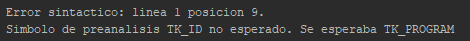
\includegraphics[scale=1]{img/sintactico/salida_sintactico_ej_error_1.png}
\caption{Salida de la ejecución del analizador sintáctico con el código de la figura \ref{fig:sintactico_ej_error_1}.}
\label{fig:sintactico_ej_error_1_salida}
\end{figure}

\begin{figure}[H]
\begin{minted}[escapeinside=||,autogobble,linenos,xleftmargin=0.35\textwidth,xrightmargin=0.35\textwidth]{pascal}
Program Example3;
Var       
    Num1, Num2, Sum : Integer;
    Result: |!Bool!|;
Begin {no semicolon}
    Sum := Num1 + Num2;
    if (Num1 > Num2) then
        Result := true
End.
\end{minted}
\caption{Programa en Pascal reducido con error sintáctico general.}
\label{fig:sintactico_ej_error_2}
\end{figure}

\begin{figure}[H]
\centering
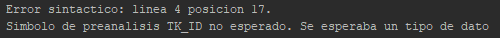
\includegraphics[scale=1]{img/sintactico/salida_sintactico_ej_error_2.png}
\caption{Salida de la ejecución del analizador sintáctico con el código de la figura \ref{fig:sintactico_ej_error_2}.}
\label{fig:sintactico_ej_error_2_salida}
\end{figure}

\begin{figure}[H]
\begin{minted}[escapeinside=||,autogobble,linenos,xleftmargin=0.35\textwidth,xrightmargin=0.35\textwidth]{pascal}
Program Example4;
|!Vars!|   
    Num1, Num2, Sum : Integer;
    Result: Boolean;
Begin {no semicolon}
    Sum := Num1 + Num2;
    if (Num1 > Num2) then
        Result := true
End.
\end{minted}
\caption{Programa en Pascal reducido con error sintáctico general y sin un token o elemento sintáctico esperado.}
\label{fig:sintactico_ej_error_3}
\end{figure}

\begin{figure}[H]
\centering
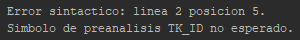
\includegraphics[scale=1]{img/sintactico/salida_sintactico_ej_error_3.png}
\caption{Salida de la ejecución del analizador sintáctico con el código de la figura \ref{fig:sintactico_ej_error_3}.}
\label{fig:sintactico_ej_error_3_salida}
\end{figure}

\section{Problemas encontrados}
Dadas las características del lenguaje, no fue posible alcanzar la clase de gramáticas LL(1), pero esto no impidió que se tomaran decisiones de diseño para poder implementar el Analizador sintáctico.

\section{Posibles mejoras}
Como mejora, en el caso de los mensajes de errores que se muestran en la compilación, debería evitarse mostrar los nombres de los tokens que se utiliza, y en su lugar deberían mostrarse los lexemas o lo que ese token representa, para ocultar aspectos de la implementación y mostrar mensajes más intuitivos.

También deberían indicarse los mensajes de error para los casos faltantes donde ``se esperaría'' un elemento sintáctico general y no un token específico.

\section{Conclusiones}
Pudimos realizar algunas modificaciones propuestas para la gramática, eliminando su recursividad a izquierda y factorizando a izquierda, pero no pudimos cumplir el requisito de que no sea ambigua, ya que el lenguaje subyacente no lo permitía. 

Más allá de no alcanzar la clase de gramáticas LL(1), el diseño y la implementación del analizador sintáctico descendente predictivo recursivo sin backtracking se pudieron concluir con éxito, tomando las decisiones pertinentes. 

Como resultado de las modificaciones sobre la gramática, ahora es más extensa y se dificulta su legibilidad y comprensión.

\chapter{Especificación semántica}
\section{Introducción}
El objetivo de este capítulo es realizar la especificación semántica del lenguaje y mostrar un pseudocódigo de su implementación.

Para llevar acabo la especificación semántica, trabajaremos sobre el analizador sintáctico de la sección anterior, realizando modificaciones que permitan implementar el analizador semántico.% utilizando una Definición Dirigida por la Sintaxis .

\section{Descripción del problema}
\label{sec:sem:descr_probl}
En esta etapa del desarrollo del compilador necesitamos extender el analizador sintáctico para poder realizar verificaciones semánticas sobre el programa a compilar. Los chequeos semánticos a realizar son:
\begin{itemize}
\item Existencia: los identificadores utilizados en el cuerpo del programa deben estar previamente declarados. El alcance de los identificadores es estático, por lo que un identificador no declarado en un ambiente se buscará en sus ambientes ancestros.
\item Unicidad: no se permite tener más de un identificador con el mismo nombre declarado en un mismo ambiente.
\item Correspondencia de parámetros: la llamada a procedimientos o funciones debe coincidir con la signatura del procedimiento o la función invocada.
\item Compatibilidad y equivalencia de tipos: los operandos de un operador deben ser compatibles para poder ejecutar correctamente la operación. %Se hará la coerción necesaria donde sea adecuado.
\end{itemize}

\section{Compatibilidad de tipos}
En la tabla \ref{tab:compatibilidad} se muestra cada operador, los tipos de los operandos que puede recibir y el tipo de resultado de la operación.

El operador ``-'' es el único operador sobrecargado, ya que puede ser utilizado tanto para operaciones binarias como unarias. En el caso de usarlo como operación unaria, su tipo de operando y resultado es el mismo que para la operación binaria. 
\begin{table}[H]
\centering
\begin{tabular}{|c|c|c|c|}
\hline
Operador                                                & Operando 1      & Operando 2      & Resultado \\ \hline
+, -,*,/                                                & Integer         & Integer         & Integer   \\ \hline
=, \textless{}\textgreater{}                            & Integer/Boolean & Integer/Boolean & Boolean   \\ \hline
\textless{},\textless{}=,\textgreater{},\textgreater{}= & Integer         & Integer         & Boolean   \\ \hline
and, or                                                 & Boolean         & Boolean         & Boolean   \\ \hline
not                                                     & Boolean         & -               & Boolean   \\ \hline
:=                                                      & Boolean         & Boolean         & -         \\ \hline
:=                                                      & Integer         & Integer         & -         \\ \hline
\end{tabular}
\caption{Compatibilidad de tipos}
\label{tab:compatibilidad}
\end{table}

\section{Estrategias}
Se utilizaron estructuras de objetos para la representación de la tabla de símbolos de manera que esta fuera fácilmente accedida por el Analizador Semántico. En tal estructura se dispusieron atributos de manera que se pueda identificar el nombre del programa, función o procedimiento que corresponde al ambiente nuevo, como también listas para los tipos de los identificadores reconocidos en su interior, y para los parámetros que recibe, en caso de que corresponda. Esto nos permitió chequear fácilmente el retorno de las funciones y las llamadas recursivas, los cuáles son casos particulares que deben tratarse.

%\section{Limitaciones}
%La estructura desarrollada para la tabla de símbolos presenta limitaciones con respecto a la expansión de los atributos que esta puede almacenar para cada identificador. Esto es debido a que se plantearon como listas de atributos solo aquellas características que se deseaban almacenar para los chequeos que se proponen en la sección \ref{sec:sem:descr_probl}. Por lo tanto si se desean agregar mas atributos, es necesario agregar nuevas listas en la estructura, donde se mapeen los identificadores a su valor de atributo, como también sus métodos de acceso correspondientes. Por ejemplo para almacenar el valor de los tipos de los identificadores en la tabla de símbolos, se utiliza una lista que mapea de identificadores a tipos, y se deben agregar todas las operaciones correspondientes para acceder a esta lista. En este sentido, el acceso a los datos de la tabla de símbolos no es genérico ya que si quiero acceder a otro dato, como los parámetros de un subprograma, debo utilizar otra operación correspondiente para tal acceso.

%esto no es una limitación, es una característica de la implementación de la TS. Desde el punto de vista del semántico la tabla de símbolos es genérica porque le provee las operaciones que necesita el semántico.

\section{Diseño del analizador semántico}
Para modelar el diseño del analizador semántico, se trabajará sobre algunas reglas de la gramática de la sección \ref{sec:gramatica_mod}, agregando acciones semánticas. Estas acciones permiten extender la potencia de las gramáticas libres de contexto, convirtiendo la gramática en una gramática de atributos.

Toda aquella información que se requiera persistir para las acciones semánticas, y que no pueda ser enviada mediante parámetros entre las llamadas de las reglas de la gramática, será almacenada en la tabla de símbolos para su posterior acceso.

\subsection{Tabla de símbolos}
La tabla de símbolos (TS) es la estructura que guarda toda la información necesaria para el proceso de análisis semántico. En este trabajo, proponemos una tabla de símbolo para cada ambiente particular.
Como el alcance de los identificadores es estático, cada identificador pertenecerá a un ambiente \emph{A}, y podrá ser accedido por aquellos ambientes \emph{A'} que estén contenidos en \emph{A}.

El Analizador Semántico mantendrá siempre una referencia a la Tabla de Símbolos del ambiente actual que esté procesando.

En la Tabla \ref{tab:tabla_simbolos} se esquematiza la forma que tendrá la tabla de símbolos explicada.

\begin{table}[H]
	\centering
	\begin{tabular}{|c|c|c|c|c|c|}
		\hline
		Ambiente & Nombre & Tipo & \multicolumn{3}{c|}{Listas de valores} \\ \hline
		\multirow{5}{*}{1} & \multirow{5}{*}{$ambiente_1$} & \multirow{5}{*}{\begin{tabular}[c]{@{}c@{}}{[}program $\lvert$ \\ function $\lvert$ \\ procedure{]}\end{tabular}} & Identificador & Tipo & Parámetros \\ \cline{4-6} 
		&  &  & $id_{var}$ & \begin{tabular}[c]{@{}c@{}}{[}integer $\lvert$ \\ boolean{]}\end{tabular} & {[} {]} \\ \cline{4-6} 
		&  &  & $id_{subprogram}$ & void & {[} $param_1$, \dots, $param_n$ {]} \\ \cline{4-6} 
		&  &  & \multicolumn{3}{c|}{\dots} \\ \cline{4-6} 
		&  &  & $id_n$ & \dots & \dots \\ \hline
		\multicolumn{6}{|c|}{\dots} \\ \hline
		n & $ambiente_n$ & \dots & \dots & \dots & \dots \\ \hline
	\end{tabular}
\caption{Esquema de la tabla de símbolos diseñada.}
\label{tab:tabla_simbolos}
\end{table}

\subsection{Gramática de atributos}
\label{sec:sem:gram_atrib}
Algunas reglas de la gramática serán alteradas para insertar y recuperar información de la tabla de símbolos, y permitirán cumplir con los objetivos propuestos en la sección \ref{sec:sem:descr_probl}.
Los siguientes no terminales se verán modificados, y sus correspondientes implementaciones en el Analizador Sintáctico cambiaran según estas modificaciones:

\begin{itemize}
\item $<$bool$>$ sintetiza el atributo \texttt{type} indicando el type boolean.
\item $<$number$>$ sintetiza el atributo \texttt{type} indicando el type integer.
\item $<$literal$>$ sintetiza el atributo \texttt{type} con el type del literal. Este valor se extrae del atributo sintetizado de $<$bool$>$ o $<$number$>$.
\item $<$factor$>$ sintetiza el atributo \texttt{type}. También verifica que pueda aplicarse el operador unario correctamente en $<$factor$>$ $\rightarrow$ $<$factor$_1$$>$ utilizando el atributo \texttt{type} de $<$factor$_1$$>$.
\item $<$identifier$>$ sintetiza el atributo \text{id} con el valor del identificador.
\item $<$type$>$ sintetiza el atributo \texttt{type} indicando el valor del tipo de dato. 
\item $<$expression-or$>$, $<$expression-and$>$, $<$expression-rel$>$, $<$expression-add$>$, $<$expression-mult$>$ y $<$factor$>$ sintetizan el atributo \texttt{type} que indica el tipo dato de la expresión.
\item $<$expression-or$_1>$, $<$expression-and$_1>$, $<$expression-rel$_1>$, $<$expression-add$_1>$, $<$expression-mult$_1>$ verifican que pueda aplicarse su operación correspondiente usando el atributo \texttt{type1} sintetizado y \texttt{type2} heredado . 
\item $<$identifier-list$>$ sintetiza el atributo \texttt{list\_id} que devuelve una lista de identificadores. Para cargar la lista utiliza el atributo sintetizado \texttt{id} de $<$identifier$>$.
\item $<$variable-declaration$>$ utiliza los atributos sintetizados \texttt{list\_id} y \texttt{type} para insertar en la tabla de símbolos cada identificador con su tipo.
\item $<$parameter-declaration$>$ sintetiza un atributo \texttt{list\_parameters} que devuelve una lista con listas de identificadores y sus tipos.
\item $<$procedure-heading$>$ utiliza el atributo sintetizado \texttt{id} y lo guarda en la tabla de simbolos. También utiliza el atributo sintetizado de $<$parameter-declaration$>$ para guardar los parámetros y sus tipos en la tabla de símbolos
\item $<$function-heading$>$ utiliza los atributos sintetizados \texttt{id} y \texttt{type} y los guarda en la tabla de símbolos. También utiliza el atributo sintetizado de $<$parameter-declaration$>$ para guardar los parámetros y sus tipos en la tabla de símbolos
\item $<$assignment-statement$>$ utiliza el atributo heredado \texttt{type} junto con el atributo sintetizado \texttt{type} de $<$expression-or$>$ para verificar si se puede efectuar la asignación.
\item $<$conditional-statement$>$ y $<$repetitive-statement$>$ utilizan el atributo sintetizado \texttt{type} de $<$expression-or$>$ para verificar que la expresión de la condición sea booleana.
\end{itemize}

\section{Implementación del aplicativo}
En esta sección mostraremos las principales modificaciones del analizador sintáctico teniendo en cuenta la gramática \ref{sec:sem:gram_atrib}. 

\subsection{Descripción del problema}
En esta etapa requerimos implementar el Analizador Semántico. Como es un análisis que debe hacerse en conjunto con el análisis sintáctico, el código del Analizador Semántico será embebido en el Analizador Sintáctico.

Cuando se encuentre un error semántico, se lanzará un error que brinde información significativa para poder corregirlo. 

\subsection{Herramientas utilizadas}
Para desarrollar el programa continuamos desde el mismo proyecto que el Analizador Sintáctico, en lenguaje Java. La versión de Java sobre la que trabajamos es la 8\footnote{Actualización 171, al día 14/05/2018}(ocho), sobre el sistema operativo Windows 10. 

\subsection{Diseño}
La idea del Analizador Semántico es modificar los procedimientos implementados del Analizador Sintáctico. Cuando un procedimiento requiera acceder a atributos sintetizados, creará variables para poder recibir los atributos; y cuando un procedimiento requiera atributos heredados, los recibirá por parámetro. 

Para no perder la implementación del Analizador Sintáctico, crearemos otra clase llamada \textbf{AnalizadorSemántico} dentro del paquete \textbf{semantico} con el mismo código del \textbf{AnalizadorSintactico}, y además crearemos el TDA \textbf{Ambiente}, por lo que nuestro árbol de directorios quedará como en la figura \ref{fig:arbol_dir_4}.

\begin{figure}[H]
%no borrar el % de dirtree porque es necesario.
\dirtree{%
.1 src.
.2 compiladorpascal.
.3 CompiladorPascal.java.
.3 lexico.
.3 sintactico.
.3 semantico.
.4 AnalizadorSemantico.java.
.4 Ambiente.java.
}
\caption{Árbol de directorios del proyecto de Java con los archivos del analizador semántico.}
\label{fig:arbol_dir_4}
\end{figure}

Para manejar los errores, creamos los métodos \texttt{errorSemantico()} y \texttt{errorSintactico()}, para que sea más fácil la invocación de errores, y se puedan mostrar mensajes adecuados.

El diseño de la tabla de símbolos se basa en guardar todo el contenido de un ambiente en su respectiva instancia del TDA \textbf{Ambiente}. Para cada ambiente del programa se guardan sus identificadores. Si el identificador es una variable o una función se le asigna su tipo, en el caso de los procedimientos se les asigna el tipo \texttt{void} por defecto. Si el identificador es una función o procedimiento, se le asocia una lista que contiene los tipos de sus parámetros manteniendo el orden en el que son declarados.

Cuando inicia el programa se crea el ambiente principal, y luego cada vez que se inicia una función o un procedimiento se crea un ambiente nuevo y se asigna como padre de este al ambiente anterior. Cuando se termina de analizar el cuerpo de un procedimiento o función, se actualiza la referencia del analizador semántico con el padre del ambiente analizado.

A continuación podemos ver la interfaz de la clase \textbf{Ambiente}.

\begin{minted}[autogobble,linenos,xleftmargin=0.025\textwidth,xrightmargin=0.025\textwidth,breaklines]{java}
public class Ambiente {
	Ambiente padre; //ambiente padre
	//puede ser program, function o procedure
	private String tipoAmbiente;
	//nombre del ambiente
	private String nombre;
	//Asocia un identificador a su type Void para procedimientos
	private HashMap<String, String> tipos;
	//Asocia un nombre de un identificador de funcion o procedimiento a su lista 
	//de parametros (solo el type de los parametros), como <nombreFuncion, parametros>
	private HashMap<String, LinkedList<String>> parametros;

	public Ambiente(String tipoAmbiente, String nombre, Ambiente padre) {}

	public Ambiente getPadre() {}

	public String getTipoAmbiente() {}

	public void setTipoAmbiente(String tipoAmbiente) { }

	public String getNombre() {}

	public HashMap<String, String> getTipos() {}

	public LinkedList<String> getParametros(String id) {}

	public void setParametros(String id, LinkedList<String> parametros) {}

	public void addParametro(String id, String tipo) {}

	public void addVariable(String id, String tipo) {}

	public void addFunction(String id, String tipo) {}

	public void addProcedure(String id) {}

	public String getTipo(String id) {}

	public boolean equals(String ident, LinkedList<String> param) {}

	public String toString() {}
}
\end{minted}

A continuación se exponen algunos fragmentos de código donde se utilizan las instancias de Ambiente para realizar las verificaciones semánticas.\\

\textbf{Declaración de variables:} cuando se encuentra una sección de declaración de variables, al insertarlas se verifican que no existan en la tabla de símbolos. Si ya existe una variable en la tabla de símbolos entonces ocurre un error de unicidad.

\begin{minted}[autogobble,linenos,xleftmargin=0.025\textwidth,xrightmargin=0.025\textwidth,breaklines]{java}
private void variable_declaration() {
	if (preanalisis.getNombre().equals("TK_ID")) {
		LinkedList<String> idents = new LinkedList<>();
		identifier_list(idents);
		match("TK_TPOINTS");
		String type = type();
		//carga los identificadores y sus tipos.
		for (String id : idents) {
			//chequear unicidad
			if (tablaActual.getTipos().containsKey(id) || tablaActual.getNombre().equals(id)) {
				errorSemantico("unicidad", id);
			} else {
				tablaActual.addIdentificador(id, type);
			}
		}
	} else {
		errorSintactico("TK_ID");
	}
}
\end{minted}

\textbf{Declaración de procedimientos:} cuando se encuentra un procedimiento se crea un nuevo ambiente. El ambiente nuevo recibe la clase de ambiente, el nombre del identificador del ambiente, y el ambiente padre. Se recorren las listas de parámetros para agregarlos a ambos ambientes, en el hijo se requieren los identificadores, y en el padre los tipos. 

\begin{minted}[autogobble,linenos,xleftmargin=0.025\textwidth,xrightmargin=0.025\textwidth,breaklines]{java}
private void procedure_heading() {
	if (preanalisis.getNombre().equals("TK_PROCEDURE")) {
		match("TK_PROCEDURE");
		String nombre = identifier();
		LinkedList<LinkedList<String>> listaParametros = new LinkedList<>();
		parameters(listaParametros);
		//se agrega el identificador al padre
		if (tablaActual.getTipos().containsKey(nombre)) {
			errorSemantico("unicidad", nombre);
		} else {
			tablaActual.addProcedure(nombre);
		}
		//se crea la nueva tabla para el ambiente actual del procedimiento
		Ambiente padre = tablaActual;
		tablaActual = new Ambiente("TK_PROCEDURE", nombre, padre);
		String id;
		String type;
		int i = 0;
		LinkedList<String> aux;
		while (i < listaParametros.size()) {
			aux = listaParametros.get(i);
			type = aux.get(0);
			for (int j = 1; j < aux.size(); j++) {
				id = aux.get(j);
				if (tablaActual.getTipos().containsKey(id) || tablaActual.getNombre().equals(id)) {
					errorSemantico("unicidad", id);
				} else {
					tablaActual.addIdentificador(id, type);
					//se le asigna al padre 
					tablaActual.getPadre().addParametro(nombre, type);
				}
			}
			i++;
		}
	} else {
		errorSintactico("TK_PROCEDURE");
	}
}
\end{minted}

\textbf{Verificación de compatibilidad de tipos:} cuando ocurre una operación se debe verificar que sus operandos se correspondan con los tipos definidos en la tabla \ref{tab:compatibilidad}. En estos casos, siempre se recibe un atributo heredado que es el tipo del primer operando, y un atributo sintetizado que es el tipo del segundo operando (con excepción de las operaciones unarias).

\begin{minted}[autogobble,linenos,xleftmargin=0.025\textwidth,xrightmargin=0.025\textwidth,breaklines]{java}
private String expression_or_1(String type) {
	if (preanalisis.getNombre().equals("TK_BOOL_OP_OR")) {
		match("TK_BOOL_OP_OR");
		String type2 = expression_and();
		if (not((type.equalsIgnoreCase(type2)) and type.equalsIgnoreCase("TK_TYPE_BOOL"))) {
			errorSemantico("type", type + " y " + type2 + " no aplicables a operador OR");
		}
		type = "TK_TYPE_BOOL";
		type = expression_or_1(type);
	}
	return type;
}
\end{minted}

Para ver el flujo de datos que ocurren durante el análisis, se muestran a continuación árboles de derivación anotados, donde se aprecia el uso de los ambientes y los atributos de la gramática  embebidos en el análisis sintáctico.

Para simplificar el nombre de los nodos, se abrevió el nombre de los no terminales de la gramática, quedando como los de la siguiente lista:
\begin{itemize}
    \item VD: Variable\_declaration
    \item IL: Identifier\_list
    \item I: Identifier
    \item IL\_1: Identifier\_list\_1
    \item VDL: variable\_declaration\_list
    \item VDL\_1: variable\_declaration\_list\_1
    \item PD: procedure\_declaration
    \item PH: procedure\_heading
    \item P: parameters
    \item P\_2: parameters\_2
    \item PDL: parameter\_declaration\_list
    \item PrD: parameter\_declaration
\end{itemize}

\begin{figure}[H]
\centering
\begin{tikzpicture}[scale=0.65, node distance = 2.5cm, state/.style={circle, draw, minimum size=1cm}]
\tikzset{every state/.append style={thick, fill=gray!10}}
\node[state] (0) at (0,6) {VD};
\node[state] (1) at (-3,4) {IL};
\node[state] (2) at (3,4) {T};
\node[state] (3) at (-1,2) {IL\_1};
\node[state] (4) at (-5,2) {I};
\node[state] (5) at (-1,0) {IL};
\node[state] (6) at (1,-2) {IL\_1};
\node[state] (7) at (-3,-2) {I};

\node[right] (8) at (6,4) {{\bf ($addAmbiente(list\_id, type)$)}};

\path[->,>=stealth]
(0) edge[above] node{$ $} (1)
    edge[above] node{$ $} (2)
    edge[bend left=25] node{$ $} (8)

(1) edge[above] node{$ $} (3)
    edge[above] node{$ $} (4)
    edge[bend left, left] node{$list\_id=\{'a','b'\}$} (0)

(2) edge[bend right, right] node{$type=integer$} (0)

(3) edge[bend right, right] node{$'b'$} (1)
    edge[above] node{$ $} (5)
    
(4) edge[bend left, left] node{$'a'$} (1)

(5) edge[above] node{$ $} (6)
    edge[above] node{$ $} (7)

(7) edge[bend left, left] node{$'b'$} (5)
   % edge[bend left, left] node{$ $} (3)
;
\end{tikzpicture}
\caption{Declaración simple de variables.}
\label{fig:arbol_declaracion_var}
\end{figure}

En la figura \ref{fig:arbol_declaracion_var} se ve un árbol de derivación anotado teniendo en cuenta la gramática de atributos  y el uso de la tabla de símbolos, para la definición de dos variables integer: ``VAR a,b:integer;''. Cuando el no terminal VD obtiene el atributo list\_id que tiene la lista de identificadores declarados y type que tiene el tipo de dato de los identificadores, puede insertarlos en el Ambiente actual, que representa la tabla de símbolos de la subrutina que está analizando.

\begin{figure}[H]
\centering
\begin{tikzpicture}
\tikzset{every state/.append style={thick, fill=gray!10}}
\node[state] (0) at (0,6) {VDL};
\node[state] (1) at (-2,4) {VD};
\node[state] (2) at (2,4) {VDL\_1};
\node[coordinate] at (-2,2) (3) {};
\node at (-2,2) [isosceles triangle, shape border rotate=+90,
draw,minimum size=8mm,minimum height=2cm,
anchor=north] (3triangle) { };
%Inserta a,b:integer como en el árbol de la fig. \ref{fig:arbol_declaracion_var}
\node[right] (5) at (-4,-0.5) {Inserta a,b:integer};
\node[right] (6) at (-4,-1) {como en el árbol de la fig. \ref{fig:arbol_declaracion_var}};

\node[state] (4) at (2,2) {VD};
\node[coordinate] at (2,0) (5) {};
\node at (2,0) [isosceles triangle, shape border rotate=+90,
draw,minimum size=8mm,minimum height=2cm,
anchor=north] (5triangle) { };
%Inserta c:boolean como en el árbol de la fig. \ref{fig:arbol_declaracion_var}
\node[right] (7) at (0,-2.5) {Inserta c:boolean};
\node[right] (8) at (0,-3) {como en el árbol de la fig. \ref{fig:arbol_declaracion_var}};

\path[->,>=stealth]
(0) edge[above] node{$ $} (1)
    edge[above] node{$ $} (2)

(1) edge[above] node{$ $} (3)

(2) edge[above] node{$ $} (4)

(4) edge[above] node{$ $} (5)
;
\end{tikzpicture}
\caption{Declaración de listas de variables.}
\label{fig:arbol_declaracion_list_var}
\end{figure}

En la figura \ref{fig:arbol_declaracion_list_var} se ve el árbol de derivación para insertar una lista de variables con la siguiente sintaxis: ``VAR a,b:integer; c:boolean''. Así, la subrutina que está siendo analizada va a recibir todas sus variables sin importar cómo sea la declaración de variables.

En el siguiente árbol de la figura \ref{fig:arbol_declaracion_param} veremos la declaración de un procedimiento con parámetros, similar a la declaración de variables pero jugando un poco más con la tabla de símbolos.

\begin{figure}[H]
	\centering
	\begin{tikzpicture}[scale=0.65, node distance = 2.5cm, state/.style={circle, draw, minimum size=1cm}]
	\tikzset{every state/.append style={thick, fill=gray!10}}
	\node[state] (0) at (0,6) {PD};
	\node[state] (1) at (0,4) {PH};
	\node[state] (2) at (-3,2.5) {I};
	\node[state] (3) at (0,1.5) {P};
	\node[state] (4) at (0,-0.5) {P\_2};
	\node[state] (5) at (0,-3) {PDL};
	\node[state] (6) at (0,-5) {PRD};
	\node[state] (7) at (-3,-7) {IL};
	\node[state] (8) at (3,-7) {T};
	\node[state] (9) at (-5,-8) {I};	
	
	\node[coordinate] at (5,3) (InsTS) {};
	\node[right] (10) at (5,3) {{\bf ($TSproc = crearTS('proc',TSPadre)$}};
	\node[right] (11) at (5,2.5) {{\bf ($addVariables(TSProc,{'a'}, 'integer')$)}};
	\node[right] (12) at (5,2) {{\bf ($addParametros(TSPadre,'proc', 'integer')$)}};
	
	\path[->,>=stealth]
	(0) edge[above] node{$ $} (1)
	
	(1) edge[above] node{$ $} (2)
	edge[above] node{$ $} (3)
	edge[bend left=25] node{$ $} (InsTS)
	
	(2) edge[bend left, left] node{$nombre='proc'$} (1)
	
	(3) edge[above] node{$ $} (4)
	edge[bend right, right] node{$\{\{'integer','a'\}\}$} (1)
	
	(4) edge[bend right, right] node{$\{\{'integer','a'\}\}$} (3)
	edge[above] node{$ $} (5)
	
	(5) edge[above] node{$ $} (6)
	edge[bend right, right] node{$\{\{'integer','a'\}\}$} (4)
	
	(6) edge[above] node{$ $} (7)
	edge[above] node{$ $} (8)
	edge[bend right, right] node{$\{\{'integer','a'\}\}$} (5)
	
	(7) edge[above] node{$ $} (9)
	 edge[bend left, left] node{$\{'a'\}$} (6)
	 
	(8) edge[bend right, right] node{$'integer'$} (6)
	 
	(9) edge[bend left, left] node{$'a'$} (7)
	% edge[bend left, left] node{$ $} (3)
	;
	\end{tikzpicture}
	\caption{Declaración simple de variables.}
	\label{fig:arbol_declaracion_param}
\end{figure}

En la figura \ref{fig:arbol_declaracion_param} se muestra el análisis para la declaración del encabezado de un procedimiento con la sintaxis: ``procedure proc(a:integer);''. El árbol muestra cómo se obtiene el nombre del procedimiento, sus parámetros y luego en el nodo PH se procede a crear la nueva tabla de símbolos para ese procedimiento, la cual recibe como parámetro el nombre del procedimiento y la tabla de símbolos del padre (teniendo en cuenta su estructura lexicográfica). Luego se agregan los parámetros como variables a la tabla del procedimiento; y se agregan los tipos de los parámetros a la tabla del procedimiento padre, para que cuando se invoque a \emph{proc}, pueda chequear la cantidad y el tipo de los parámetros que se le envían.

Si la declaración de parámetros fuera la siguiente: (a,b:integer;c:boolean), en el nodo PRD se armaría la siguiente lista: \{\{'integer','a','b'\},\{'boolean','c'\}\}, y una vez que llegue a PH se ejecutaría \\ 
addVariables(TSProc,'a','integer'), addVariables(TSProc,'b','integer'), addVariables(TSProc,'c','boolean') y \\ addParametros(TSPadre,'proc',\{'integer','integer','boolean'\}). 

\subsection{Instructivos de instalación y uso}
Para usar el programa es idéntico que para el Análizador Sintáctico, al ser un programa portable, solo se requiere la compilación a través del comando \emph{javac *.java} o cargando el proyecto en el NetBeans y usando este para compilar.

Para ejecutar, hay que invocar el programa compilado enviándole como parámetro el archivo con el código fuente del programa a compilar.

También es posible ejecutar la batería de ejemplos mediante el ejecutable \texttt{bateria-wind.bat} para Windows o \texttt{bateria-linux.sh} para Linux.

\subsection{Ejemplos}
Para mostrar el funcionamiento del Analizador Semántico proponemos una serie de ejemplos para demostrar las funcionalidades semánticas implementadas.

%unicidad
\subsubsection{Chequeo de unicidad}
\begin{figure}[H]
\begin{minted}[escapeinside=||,autogobble,linenos,xleftmargin=0.35\textwidth,xrightmargin=0.35\textwidth]{pascal}
Program Example1;
Var       
    Num1, Num2, Sum1 : Integer;
    |!Num1!|: Boolean;
Begin
    Sum := Num1 + Num2;
    if (Num1 > Num2) then
        Result := true
End.
\end{minted}
\caption{Programa en Pascal reducido con error de unicidad en variable Num1.}
\label{fig:semantico_ej_error_1}
\end{figure}

\begin{figure}[H]
\centering
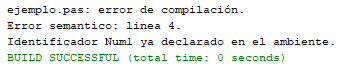
\includegraphics[]{img/semantico/semantico_ej1.png}
\caption{Resultado compilación ejemplo1.}
\label{fig:semantico_ej1}
\end{figure}

%existencia \(declaración de variable\)
\subsubsection{Chequeo de existencia}
\begin{figure}[H]
\begin{minted}[escapeinside=||,autogobble,linenos,xleftmargin=0.35\textwidth,xrightmargin=0.35\textwidth]{pascal}
Program Example2;
Var       
    Num1, Num2, Sum1 : Integer;
Begin 
    Num1 := 2;
    |!Sum2!| := Num1 + Num2;
End.
\end{minted}
\caption{Programa en Pascal reducido con falta de declaración de variable Sum2.}
\label{fig:semantico_ej_error_2}
\end{figure}

\begin{figure}[H]
\centering
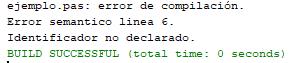
\includegraphics[]{img/semantico/semantico_ej2.png}
\caption{Resultado compilación ejemplo2.}
\label{fig:semantico_ej2}
\end{figure}

%correspondencia de parametros en llamada a funcion
\subsubsection{Correspondencia de parámetros}
\begin{figure}[H]
\begin{minted}[escapeinside=||,autogobble,linenos,xleftmargin=0.35\textwidth,xrightmargin=0.35\textwidth]{pascal}
Program Example3;
Var       
    Num1, Num2, Sum1 : Integer;
    Procedure proc(a:integer, b:boolean);
    begin
        b := true;
    end;
Begin
    proc(Num1,true);
    |!proc(Num1,Num2)!|
End.
\end{minted}
\caption{Programa en Pascal reducido con error en la llamada al procedimiento proc en la línea 10.}
\label{fig:semantico_ej_error_3}
\end{figure}

\begin{figure}[H]
\centering
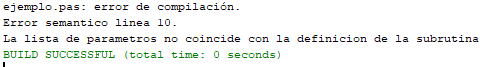
\includegraphics[]{img/semantico/semantico_ej3.png}
\caption{Resultado compilación ejemplo3.}
\label{fig:semantico_ej3}
\end{figure}

%uso de identificador funcion para devolver su resultado 
\subsubsection{Devolver valor de una función}
\begin{figure}[H]
\begin{minted}[escapeinside=||,autogobble,linenos,xleftmargin=0.35\textwidth,xrightmargin=0.35\textwidth]{pascal}
Program Example4;
Var       
    Num1, Num2, Sum1 : integer;
    function f1(a:integer): integer ;
    begin
        |!f1!| := a+3;
    end;
Begin
    f1(Num1)
End.
\end{minted}
\caption{Programa en Pascal reducido con uso de identificador f1 para devolver un valor.}
\label{fig:semantico_ej_error_4}
\end{figure}

\begin{figure}[H]
\centering
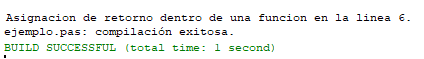
\includegraphics[]{img/semantico/semantico_ej4.png}
\caption{Resultado compilación ejemplo4.}
\label{fig:semantico_ej4}
\end{figure}

%compatibilidad de tipos para asignacion
\subsubsection{Compatibilidad de tipos}

\begin{figure}[H]
\begin{minted}[escapeinside=||,autogobble,linenos,xleftmargin=0.35\textwidth,xrightmargin=0.35\textwidth]{pascal}
Program Example5;
Var       
    Num1, Num2, Sum1 : Integer;
    Procedure proc(a:integer, b:boolean);
    begin
        a := 3;
        |!b := a;!|
    end;
Begin
    proc(Num1,Num2)
End.
\end{minted}
\caption{Programa en Pascal reducido con error en la compatibilidad de tipos línea 7.}
\label{fig:semantico_ej_error_5}
\end{figure}

\begin{figure}[H]
\centering
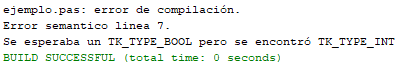
\includegraphics[]{img/semantico/semantico_ej5.png}
\caption{Resultado compilación ejemplo5.}
\label{fig:semantico_ej5}
\end{figure}

%\section{Problemas encontrados}
%ni ahi

%\section{Posibles mejoras}
%ninguna

\section{Conclusión}
Cumplimos con los requerimientos propuestos en la descripción del problema \ref{sec:sem:descr_probl}, extendiendo el Analizador Sintáctico con las reglas semánticas y utilizando los atributos descritos en \ref{sec:sem:gram_atrib}. 


\chapter{Generación de código intermedio}

\section{Introducción}
Luego de realizar todos los chequeos sintácticos y semánticos propuestos, llega la etapa de generar código ejecutable.

En este capítulo desarrollaremos la especificación y la implementación de la generación de código intermedio del lenguaje, utilizando código de tres direcciones, y generando un código ejecutable por una máquina virtual.

\section{Descripción del problema}
\label{sec:gen_cod:descr_prob}
En esta etapa necesitamos traducir las sentencias del lenguaje pascal a instrucciones de bajo nivel. Para esto, nuestro lenguaje intermedio será MEPa, cuyas instrucciones son ejecutables por la máquina virtual MEPa. 

El objetivo es ampliar la funcionalidad del analizador semántico, embebiéndole sentencias para la generación de instrucciones MEPa.

El resultado de la compilación debe ser un archivo con el código MEPa que resulte equivalente al código en lenguaje Pascal y permita la ejecución del mismo.

\section{Máquina virtual MEPa}
MEPa es una máquina hipótetica desarrollada teniendo en cuenta las construcciones de Pascal. Nos permite generar código ejecutable sin necesidad de tener en cuenta las particularidades y complejidad de una máquina real.

La memoria de MEPa se divide en tres secciones: la región del programa, donde almacenará el código del programa; un vector de direcciones base (display) que tendrá punteros a direcciones de la tercer región, la pila, donde almacenará los datos que serán utilizados por las operaciones. 

El uso de una pila nos permite implementar fácilmente la evaluación de expresiones, ya que la precedencia de operadores queda implícita por el recorrido del árbol de derivación que surge de nuestra sintaxis. Además, la implementación de las llamadas recursivas también se beneficia al utilizar una estructura de pila para almacenar los valores y las direcciones de retorno.

En la tabla \ref{tab:instr_mepa} se ven las instrucciones que utilizamos y su funcionalidad.

\begin{table}[]
    \centering
    \begin{tabular}{|c|c|c|}
\hline
 & Instrucción & Descripción \\ \hline
\multirow{4}{*}{\begin{tabular}[c]{@{}c@{}}Operaciones \\ aritméticas\end{tabular}} & SUMA & sumar \\ \cline{2-3} 
 & SUST & restar \\ \cline{2-3} 
 & MULT & multiplicar \\ \cline{2-3} 
 & DIVI & dividir \\ \hline
\multirow{6}{*}{\begin{tabular}[c]{@{}c@{}}Operaciones \\ relacionales\end{tabular}} & CMIG & igual \\ \cline{2-3} 
 & CMDG & desigual \\ \cline{2-3} 
 & CMME & menor \\ \cline{2-3} 
 & CMNI & menor igual \\ \cline{2-3} 
 & CMMA & mayor \\ \cline{2-3} 
 & CMYI & mayor igual \\ \hline
\multirow{2}{*}{\begin{tabular}[c]{@{}c@{}}Operaciones\\ unarias\end{tabular}} & NEGA & negación lógica \\ \cline{2-3} 
 & UMEN & menos unario \\ \hline
\multirow{2}{*}{\begin{tabular}[c]{@{}c@{}}Operaciones \\ lógicas\end{tabular}} & CONJ & and \\ \cline{2-3} 
 & DISJ & or \\ \hline
 \end{tabular}
 \begin{tabular}{|c|c|c|}
 \hline
 & Instrucción & Descripción \\ \hline
\multirow{2}{*}{\begin{tabular}[c]{@{}c@{}}Salto\\ condicional\end{tabular}} & DSVS label & desviar siempre \\ \cline{2-3} 
 & DSVF label & desviar si el tope es falso \\ \hline
\multirow{2}{*}{Apilar} & APCT c & apilar constante \\ \cline{2-3} 
 & APVL m,n & apilar variable \\ \hline
Almacenar & ALVL m,n & \begin{tabular}[c]{@{}c@{}}almacena el tope de \\ la pila en una variable\end{tabular} \\ \hline
\multirow{2}{*}{Entrada/Salida} & IMPR & imprimir por pantalla \\ \cline{2-3} 
 & LEER & leer entrada \\ \hline
\multirow{7}{*}{\begin{tabular}[c]{@{}c@{}}Programas y \\ procedimientos\end{tabular}} & INPP & inicio del programa \\ \cline{2-3} 
 & LLPR label & llamada a subrutina \\ \cline{2-3} 
 & ENPR k & entrada a procedimiento \\ \cline{2-3} 
 & RTPR k,n & \begin{tabular}[c]{@{}c@{}}retornar desde un \\ procedimiento\end{tabular} \\ \cline{2-3} 
 & RMEM c & reservar memoria \\ \cline{2-3} 
 & LMEM c & liberar memoria \\ \cline{2-3} 
 & PARA & detiene la máquina MEPa \\ \hline
 & NADA & sin efecto en la ejecución \\ \hline
\end{tabular}
    \caption{Instrucciones MEPa}
    \label{tab:instr_mepa}
\end{table}

\section{Estrategias}
Para facilitar el trabajo con los saltos condicionales de MEPa, almacenamos los \emph{labels} de cada ambiente en la tabla de símbolos.

Como no tuvimos que preocuparnos por el tamaño de los tipos de datos, para calcular los offsets de las variables utilizamos su posición en el orden de declaración, y se guardó esta posición para cada variable en la tabla de símbolos. Para calcular la memoria a reservar, contamos la cantidad de variables que había en el ambiente.

\section{Limitaciones}
Algunas operaciones de MEPa no fueron utilizadas, como salidas por pantalla o lecturas de teclado que generen saltos de línea automáticos; aunque sean más una comodidad para el programador que una limitación. 

\section{Diseño del generador de código intermedio}
Para especificar cómo se llevará a cabo la generación de código intermedio, se describirán las modificaciones necesarias sobre las reglas de la gramática.

Para cumplir los objetivos de \ref{sec:gen_cod:descr_prob}, se utilizará una variable a la cuál se le agregará el código MEPa que se genere durante la compilación. Una vez concluida la compilación el contenido de la variable se escribirá en un archivo.

\subsection{Modificaciones a la tabla de símbolos}
\label{sec:gen_cod:mod_tab_sim}
La tabla de símbolos será actualizada con nuevos valores necesarios para la generación de código intermedio. Estos valores están asociados a la profundidad y desplazamiento de los identificadores, necesarios para implementar el alcance estático a través del vector de direcciones y la pila de MEPa.

\subsection{Modificaciones a las reglas de la gramática}
Cada regla que esté asociada a la generación de instrucciones de la tabla \ref{tab:instr_mepa}, será modificada, agregándole a la variable que contiene el código MEPa la instrucción correspondiente.

\begin{itemize}
\item $<$program$>$ agrega \texttt{INPP} antes de llamar a $<$program-heading$>$  y luego de unificar con el ``.'' final agrega \texttt{PARA}. Esto indica el comienzo y fin del programa principal.
\item En $<$block$>$, luego de llamar $<$declaration-block$>$ y $<$multiple-statement$>$ agrega \texttt{LMEM X}. Esto libera la memoria asignada a las variables, donde \texttt{X} es la cantidad de variables que se reservaron en $<$declaration-block$>$.
\item $<$declaration-block$>$ agrega \texttt{RMEM X} luego de $<$variable-declaration-block$>$, reservando  \texttt{X} posiciones de memoria para las variables locales.
\item $<$procedure-declaration$>$ y $<$function-declaration$>$, agrega \texttt{DSVS LX$_{1}$} la cuál es una instrucción de salto, y donde \texttt{X$_{1}$} es un label que corresponde con el final del subprograma. Luego agrega \texttt{LX$_{2}$ ENPR P} que indica el comienzo del subprograma, y donde \texttt{X$_{2}$} es un label que se utilizará para llamar al subprograma posteriormente y \texttt{P} es la profundidad del ambiente actual. Finalmente se agrega \texttt{RTPR P X$_{3}$} y \texttt{LX$_{1}$ NADA}, para indicar el retorno del subprograma, donde \texttt{P} es la misma profundidad mencionada anteriormente, \texttt{X$_{3}$} es la cantidad de parámetros recibidos por el subprograma, y por último \texttt{X$_{1}$} es el label definido para el final del subprograma y donde se desviará la primera vez, durante la definición.
%crean las etiquetas correspondientes para marcar el comienzo y fin del procedimiento/función, para saltar el cuerpo del procedimiento/función, y para retornar el control a quien lo invocó.
\item $<$assignment-statement$>$ agrega \texttt{ALVL P O} que permite almacenar el valor del tope de la pila en una variable indicada mediante la profundidad \texttt{P} y el offset \texttt{O}.
\item  $<$call-procedure-or-function$>$ agrega varias instrucciones diferentes dependiendo del tipo de subprograma llamado:
\begin{itemize}
	\item Si es un procedimiento $write$ agrega \texttt{IMPR} que permite imprimir por pantalla el contenido del tope de la pila.
	\item Si es un procedimiento $read$ agrega \texttt{LEER} que activa la entrada por teclado y luego realiza \texttt{ALVL P O} para almacenar el valor leído en la variable indicada por la profundidad \texttt{P} y el offset \texttt{O}.
	\item Si es un procedimiento definido por el usuario, agrega \texttt{LLPR LX} que indica la llamada al procedimiento que fue etiquetado con el label \texttt{X}.
	\item Si es una función definida por el usuario, agrega \texttt{LLPR LX} que indica la llamada a la función que fue etiquetado con el label \texttt{X} y además agrega \texttt{RMEM 1} para reservar una posición de memoria extra para guardar el valor de retorno de la función.
\end{itemize}
\item $<$conditional-statement$>$ agrega \texttt{DSVF LX$_{1}$} que permite saltar el código hasta la instrucción etiquetada con \texttt{X$_{1}$} si el tope de la pila es falso, es decir no ejecuta el cuerpo del $then$ en caso de ser falsa la condición de $if$.
\item $<$else-statement$>$ agrega \texttt{DSVS LX$_{2}$} para desviar el cuerpo del $else$ en caso de que el contenido del $then$ se haya ejecutado. Luego del desvió agrega \texttt{LX$_{1}$ NADA} que será donde se desviará en caso de que el $then$ sea falso, y permitirá la ejecución del $else$, ya que este no será desviado. Finalmente agrega \texttt{LX$_{2}$ NADA} que será donde se desviará el $else$ en caso de no cumplirse. Si no se detecto la sentencia $else$ por el analizador sintáctico solo se agrega \texttt{LX$_{1}$ NADA} que corresponde a donde se desviará el $then$ en caso de ser falso.
%agrega las instrucciones para desviar el flujo de ejecución y no ejecutar el cuerpo del ``else'' si ya ejecutó el ``then''.
\item $<$repetitive-statement$>$ agrega \texttt{LX$_{1}$ NADA} que será la instrucción etiquetada donde se desviará el flujo en caso de que la condición de repetición se cumpla. Luego agrega \texttt{DSVF LX$_{2}$} y \texttt{DSVS LX$_{1}$} indicando que se desviará a la instrucción etiquetada \texttt{X$_{2}$} en caso de no cumplirse la condición del $while$ o se desviará a \texttt{X$_{1}$} en caso de cumplirse. Finalmente se agrega \texttt{LX$_{2}$ NADA} que es la instrucción a la que se desviará el flujo en caso de que no se cumpla la condición de repetición.
%agrega las instrucciones para repetir el cuerpo del ``while'' mientras se cumpla la condición.
\item $<$expression-or-1$>$ agrega \texttt{DISJ} que indica la disyunción entre los últimos dos valores booleanos almacenados en el tope de la pila.
\item $<$expression-and-1$>$ agrega \texttt{CONJ} que indica la conjunción entre los últimos dos valores booleanos almacenados en el tope de la pila.
\item $<$expression-rel-1$>$ agrega varias instrucciones diferentes dependiendo de la operación relacional que se realiza utilizando los últimos dos valores booleanos o enteros almacenados en el tope de la pila:
\begin{itemize}
	\item Agrega \texttt{CMIG} para la relación igual.
	\item Agrega \texttt{CMDG} para la relación desigual.
	\item Agrega \texttt{CMME} para la relación menor.
	\item Agrega \texttt{CMMA} para la relación mayor.
	\item Agrega \texttt{CMNI} para la relación menor igual.
	\item Agrega \texttt{CMYI} para la relación mayor igual.
\end{itemize}
\item $<$expression-add-1$>$ agrega \texttt{SUMA} o \texttt{SUST} para el caso de la operación suma o resta, según corresponda, entre los últimos dos valores enteros almacenados en el tope de la pila.
\item $<$expression-mult-1$>$ agrega \texttt{MULT} o \texttt{DIVI} para el caso de la operación multiplicación o división, según corresponda, entre los últimos dos valores enteros almacenados en el tope de la pila.
\item $<$factor$>$ agrega \texttt{UMEN} o \texttt{NEGA} para el caso de la operación unaria negación aritmética o negación relacional, según corresponda, entre los últimos dos valores enteros o booleanos almacenados en el tope de la pila. En caso de que el factor sea un identificador de variable o parámetro agrega \texttt{APVL P O} con la profundidad \texttt{P} y el offset \texttt{O} correspondiente a tal variable o parámetro para almacenar tal valor en el tope de la pila.
\item $<$number$>$ agrega \texttt{APCT C} que almacena una constante numérica \texttt{C} en el tope de la pila.
\item $<$bool$>$ agrega \texttt{APCT 1} o \texttt{APCT 0} según sea un valor constante $true$ o $false$ correspondientemente, lo cuál almacena tal valor en el tope de la pila.
\end{itemize}

\section{Implementación del aplicativo}

\subsection{Descripción del problema}
En esta implementación debemos generar el código intermedio según las sentencias del archivo de entrada en lenguaje Pascal. 

En esta etapa no existen errores de generación de código, ya que simplemente es devolver una secuencia de instrucciones, por lo que los únicos errores que lanzará el compilador son los de las etapas previas de análisis del código fuente. Si existe un error en alguna de las etapas de análisis, no se geenerará ningún archivo de salida con código MEPa.

La implementación se basará en agregar las sentencias necesarias para crear el archivo de salida con el código MEPa. Estas sentencias estarán embebidas en el analizador semántico.

\subsection{Herramientas utilizadas}
Continuamos utilizando el mismo proyecto del analizador semántico, en lenguaje Java con la misma versión y Sistema Operativo Windows 10.

Para verificar el funcionamiento del código MEPa generado, utilizamos el aplicativo que se encuentra en la plataforma PEDCo.

\subsection{Diseño}
Como la generación de código es simplemente agregar las instrucciones MEPa a una variable, y luego retornar la variable, trabajaremos sobre los procedimientos implementados en el Analizador Semántico. 

Para no perder la implementación del Analizador Semántico, crearemos otra clase llamada \textbf{GeneradorCodigoIntermedio} dentro del paquete \textbf{codigointermedio} con el mismo código del \textbf{AnalizadorSemántico}, y además crearemos otro TDA \textbf{Ambiente} modificado, por lo que nuestro árbol de directorios quedará como en la figura \ref{fig:arbol_dir_5}.

\begin{figure}[H]
%no borrar el % de dirtree porque es necesario.
\dirtree{%
.1 src.
.2 compiladorpascal.
.3 CompiladorPascal.java.
.3 lexico.
.3 sintactico.
.3 semantico.
.3 codigointermedio.
.4 GeneradorCodigoIntermedio.java.
.4 Ambiente.java.
}
\caption{Árbol de directorios del proyecto de Java con los archivos del generador de código intermedio.}
\label{fig:arbol_dir_5}
\end{figure}

La tabla de símbolos requirió agregar información tanto para poder representar el alcance estático, como para identificar qué identificadores dentro de un ambiente son variables y cuáles son parámetros, para poder calcular el correcto acceso de los valores de la pila. A continuación se puedne ver las modificaciones sobre el TDA Ambiente, donde se aprecia la información necesaria descrita en \ref{sec:gen_cod:mod_tab_sim}.

\begin{minted}[escapeinside=~~,autogobble,linenos,xleftmargin=0.025\textwidth,xrightmargin=0.025\textwidth,breaklines]{java}
public class Ambiente {
    
    ~\dots~
    
    //profundidad del ambiente
    private int profundidad = -1;
    //ultimo offset utilizado para una variable
    private int lastOffset = 0;
    //ultimo offset utilizado para un parametro
    private int lastParameterOffset = -3;
    //offset utilizado para el retorno de una funcion
    private int returnOffset = -4;
    //label de llamada para un procediemiento o funcion
    private int label = -1;
    
    //Asocia un identificador (variable) a su profundidad
    private HashMap<String, Integer> profundidades;
    //Asocia un identificador (variable) a su offset
    private HashMap<String, Integer> offsets;
    //Asocia un identificador a su clase (variable, parametro, funcion, procedimiento)
    private HashMap<String, String> clases;
    //Asocia un identificador de procedimiento o funcion a su label de llamada
    private HashMap<String, Integer> labels;
    
    ~\dots~
    
    //Asocia un identificador a su type y profundidad.
    public void addVariable(String id, String tipo, int profundidad, boolean isParameter) {
        tipos.put(id.toUpperCase(), tipo.toUpperCase());
        profundidades.put(id.toUpperCase(), profundidad);
        if (isParameter) {
            offsets.put(id.toUpperCase(), lastParameterOffset++);
            clases.put(id.toUpperCase(), "parametro");
        } else {
            offsets.put(id.toUpperCase(), lastOffset++);
            clases.put(id.toUpperCase(), "variable");
        }
    }
    ~\dots~
}
\end{minted}

Como los parámetros son enviados desde el llamador, la subrutina invocada debe acceder a ellos con un offset negativo (desde el comienzo de su registro de activación accede a posiciones anteriores de la pila), mientras que para acceder a las variables locales, debe acceder con un offset positivo (dentro de su espacio local de la pila). Por esto, al agregar esta información en la tabla de símbolos, necesitamos discriminar la clase del identificador. Esta funcionalidad se agregó al método \emph{addVariable()} utilizando un parámetro más que indica si la variable insertada es un parámetro.

Para mostrar el uso de la nueva información de la tabla de símbolos se expondrán fragmentos de los procedimientos más importantes.
\begin{minted}[escapeinside=~~,autogobble,linenos,xleftmargin=0.025\textwidth,xrightmargin=0.025\textwidth,breaklines]{java}
 private String factor() {
    ~\dots~
    if (ambiente.getClase(id).equals("variable") || ambiente.getClase(id).equals("parametro")) {
        mepa += "APVL " + ambiente.getProfundidad(id) + " " + ambiente.getOffset(id) + "\n";
        } else {
            if (ambiente.getClase(id).equalsIgnoreCase("funcion")) {
                call_procedure_or_function(id);
            } else {
            errorSemantico("bad_uso_proc", "No se permite uso de procedimientos en expresiones. Causa: retorno void.");
            }
      ~\dots~
}
\end{minted}

En el procedimiento \emph{factor()} se puede apreciar el uso de la clase de un identificador para verificar si es una variable o un parámetro, y cómo se accede a su profundidad y offset para almacenar su valor en la pila con la instrucción APVL. 



\subsection{Instructivos de instalación y uso}
La instalación y uso es idéntica que para el analizador semántico. Se puede compilar a través del comando \emph{javac *.java} o cargando el proyecto en NetBeans y utilizando este para compilar.

Para ejecutar, se debe invocar el programa compilado enviándole como parámetro el archivo con el código fuente del programa a compilar. 

Como resultado de una compilación exitosa, se debe obtener un archivo de salida con el código MEPa listo para ejecutar en la máquina virtual.

\subsection{Ejemplos}

\subsubsection{Asignación y expresión simple}
\begin{figure}[H]
\begin{minted}[escapeinside=||,autogobble,linenos,xleftmargin=0.35\textwidth,xrightmargin=0.35\textwidth]{pascal}
Program MepaExpresion;
Var
    a, b, c : integer;
Begin
    a := a + (b / 9 - 3) * c
End.
\end{minted}
\caption{Programa en Pascal reducido ilustrando una asignación de una expresión simple.}
\label{fig:ej_expresion}
\end{figure}

\begin{figure}[H]
\begin{multicols}{2}
\begin{minted}[autogobble,linenos,xleftmargin=0.2\textwidth,xrightmargin=0.2\textwidth]{xml}
INPP
RMEM 3
APVL 0 0
APVL 0 1
APCT 9
DIVI
APCT 3
SUST
APVL 0 2
MULT
SUMA
ALVL 0 0
LMEM 3
PARA
\end{minted}
\end{multicols}
\caption{Salida de la ejecución del generador de código intermedio con el código de la figura \ref{fig:ej_expresion}.}
\label{fig:gen_ej_expresion}
\end{figure}

\subsubsection{Variables locales de un subprograma}
\begin{figure}[H]
\begin{minted}[escapeinside=||,autogobble,linenos,xleftmargin=0.35\textwidth,xrightmargin=0.35\textwidth]{pascal}
Program MepaProcedimiento;
Var
    k:integer;
procedure p (n:integer; g:integer);
Var 
    h:integer;
Begin
    if n<2 then h:=g+n
    else begin
        h:=g;
        p(n-1,h);
        k:=h;
        p(n-2,g)
    end;
    write(n)
End;
Begin
    k:=0;
    p(3,k)
End.
\end{minted}
\caption{Programa en Pascal reducido ilustrando la definición y llamada de un procedimiento.}
\label{fig:ej_procedimiento}
\end{figure}

\begin{figure}[H]
\begin{multicols}{4}
\begin{minted}[autogobble,linenos,xleftmargin=0.05\textwidth,xrightmargin=0.05\textwidth]{xml}
INPP
RMEM 1
DSVS L1
L2 ENPR 1
RMEM 1
APVL 1 -4
APCT 2
CMME
DSVF L3
APVL 1 -3
APVL 1 -4
SUMA
ALVL 1 0
DSVS L4
L3 NADA
APVL 1 -3
ALVL 1 0
APVL 1 -4
APCT 1
SUST
APVL 1 0
LLPR L2
APVL 1 0
ALVL 0 0
APVL 1 -4
APCT 2
SUST
APVL 1 -3
LLPR L2
L4 NADA
APVL 1 -4
IMPR
LMEM 1
RTPR 1 2
L1 NADA
APCT 0
ALVL 0 0
APCT 3
APVL 0 0
LLPR L2
LMEM 1
PARA
\end{minted}
\end{multicols}
\caption{Salida de la ejecución del generador de código intermedio con el código de la figura \ref{fig:ej_procedimiento}.}
\label{fig:gen_ej_procediemiento}
\end{figure}

\subsubsection{Pasaje de parámetros para una función}
El pasaje de parámetros para una función es similar al de un procedimiento, con la diferencias que se reserva un lugar de memoria más en la pila antes de efectuar la llamada, para obtener el resultado de la función. Esta posición de memoria extra puede verse como un parámetro adicional, que no se desapila luego del retorno de la función.

\begin{figure}[H]
\begin{minted}[escapeinside=||,autogobble,linenos,xleftmargin=0.35\textwidth,xrightmargin=0.35\textwidth]{pascal}
Program MepaFuncion;
Var
    a: integer;
function fact(n:integer):integer;
Begin
    if n < 2 then fact := 1
    else fact := fact(n-1)*n
End;
Begin
    a:=3;
    write (fact(a))
End.
\end{minted}
\caption{Programa en Pascal reducido ilustrando la definición y llamada de una función.}
\label{fig:ej_funcion}
\end{figure}

\begin{figure}[H]
\begin{multicols}{3}
\begin{minted}[autogobble,linenos,xleftmargin=0.1\textwidth,xrightmargin=0.1\textwidth]{xml}
INPP
RMEM 1
DSVS L1
L2 ENPR 1
APVL 1 -3
APCT 2
CMME
DSVF L3
APCT 1
ALVL 1 -4
DSVS L4
L3 NADA
RMEM 1
APVL 1 -3
APCT 1
SUST
LLPR L2
APVL 1 -3
MULT
ALVL 1 -4
L4 NADA
RTPR 1 1
L1 NADA
APCT 3
ALVL 0 0
RMEM 1
APVL 0 0
LLPR L2
IMPR
LMEM 1
PARA
\end{minted}
\end{multicols}
\caption{Salida de la ejecución del generador de código intermedio con el código de la figura \ref{fig:ej_funcion}.}
\label{fig:gen_ej_funcion}
\end{figure}

\subsubsection{Sentencia condicional}
\begin{figure}[H]
\begin{minted}[escapeinside=||,autogobble,linenos,xleftmargin=0.35\textwidth,xrightmargin=0.35\textwidth]{pascal}
Program MepaCondicional;
Var
    a, b : integer;
    p, q: boolean;
Begin
    if a > b then q := p and q
        else if (a < 2*b) then p := true
            else q := false
End.
\end{minted}
\caption{Programa en Pascal reducido ilustrando una sentencia condicional.}
\label{fig:ej_if_then_else}
\end{figure}

\begin{figure}[H]
\begin{multicols}{3}
\begin{minted}[autogobble,linenos,xleftmargin=0.1\textwidth,xrightmargin=0.1\textwidth]{xml}
INPP
RMEM 4
APVL 0 0
APVL 0 1
CMMA
DSVF L1
APVL 0 2
APVL 0 3
CONJ
ALVL 0 3
DSVS L2
L1 NADA
APVL 0 0
APCT 2
APVL 0 1
MULT
CMME
DSVF L3
APCT 1
ALVL 0 2
DSVS L4
L3 NADA
APCT 0
ALVL 0 3
L4 NADA
L2 NADA
LMEM 4
PARA
\end{minted}
\end{multicols}
\caption{Salida de la ejecución del generador de código intermedio con el código de la figura \ref{fig:ej_if_then_else}.}
\label{fig:gen_ej_if_then_else}
\end{figure}

\subsubsection{Sentencia repetitiva}

\begin{figure}[H]
\begin{minted}[escapeinside=||,autogobble,linenos,xleftmargin=0.35\textwidth,xrightmargin=0.35\textwidth]{pascal}
Program MepaRepetitiva;
Var
    s, n : integer;
Begin
    while s <= n do
        s := s + 3
End.
\end{minted}
\caption{Programa en Pascal reducido ilustrando una sentencia repetitiva.}
\label{fig:ej_while_do}
\end{figure}

\begin{figure}[H]
\begin{multicols}{2}
\begin{minted}[autogobble,linenos,xleftmargin=0.2\textwidth,xrightmargin=0.2\textwidth]{xml}
INPP
RMEM 2
L1 NADA
APVL 0 0
APVL 0 1
CMNI
DSVF L2
APVL 0 0
APCT 3
SUMA
ALVL 0 0
DSVS L1
L2 NADA
LMEM 2
PARA
\end{minted}
\end{multicols}
\caption{Salida de la ejecución del generador de código intermedio con el código de la figura \ref{fig:ej_while_do}.}
\label{fig:gen_ej_while_do}
\end{figure}

\section{Problemas encontrados}
Durante la generación de funciones, nos encontramos que si una función era llamada y su valor de retorno no era usado, la pila de MEPa quedaba con memoria reservada, lo que generaba problemas cuando se hacían retornos al procedimiento llamador. Por esto, evitamos el uso de funciones cuyo valor de retorno no sea usado.

\section{Posibles mejoras}
Puede realizarse una optimización de las instrucciones generadas, sobre todo si se encuentra algún flujo del programa que nunca se ejecute, por ejemplo en una sentencia condicional con la forma if (false) \{instrucciones...\}.

\section{Conclusión}
Pudimos generar el código intermedio MEPa cumpliendo todas las características propuestas. El conjunto de instrucciones resultante no está optimizado, por lo que pueden haber instrucciones innecesarias que reduzcan la eficiencia del programa.

Como consecuencia de trabajar sobre el mismo código que el Analizador Semántico, el programa creció y se dificulta su lectura.



\end{document}